\documentclass[12pt,oneside,a4paper]{report}
\usepackage{mathtools}
\usepackage[HTML, hyperref, svgnames, table]{xcolor}
\usepackage[utf8]{inputenc}
\usepackage{multicol}
\usepackage{graphicx} 
\usepackage[margin=1in]{geometry}
\usepackage[linesnumbered,ruled,vlined]{algorithm2e}
\usepackage{booktabs}
\usepackage{tabularx}
\usepackage{algpseudocode}
\usepackage[]{algorithm2e}
\usepackage{diagbox}
\usepackage{makecell}
\usepackage[justification=centering]{caption}
\usepackage{pdfpages}

\begin{document}

\includepdf[pages=1]{./img/tutul.pdf}
\includepdf[pages=2]{}


\vspace{2cm}
\section*{Abstract}

The main goal of the thesis is to present author's implementation of the Deep CFR algorithm with the
Heads Up Limit Poker Texas Hold'em. It is a modern method for creating artificial intelligence in large partial-observable games. Such environments
have always been a great challenge and the main barrier to the development of machine learning. The thesis will show this problem by implementation of Deep CFR and analysis of the results.
For this purpose, five recognition models were created every 10 iterations of the algorithm. 
The next step was to create games with that models. The results allowed to select the best playing models and to see how Deep CFR learned over time.
Additionally, the quality of the models was tested against a simple program which simulate beginner player.

\includepdf[pages=4]{}

%\shipout\null

\newgeometry{top=2.5cm,bottom=2.5cm,right=2.5cm,left=2.5cm}
\tableofcontents{}
\newpage
\includepdf[pages=6]{}
\setlength{\parindent}{0.5em}
\setlength{\parskip}{0.5em}
\renewcommand{\baselinestretch}{1.5}



\chapter{Introduction}

Machine learning has been in development for a long time.
As early as the 40s, books and programs related to artificial intelligence \cite{hist AI}
have been writting. 
In 1940 Donald Hebb created theoretical foundations used in 
modern neural networks \cite{hist AI}. Despite such early progress, the branch of
science,
has begun to achieve great success about 10 years ago. This is due to the fact that many algorithms
need
a lot of computational power \cite{hist AI}.  

Today, there are many tools under development which are related with this topic.
For example voice assistants, language translators, models to display elements on
websites, video games or smart cars.
Additionaly, artificial intelligence is heavily used in companies,
on production halls, in transportation, medicine or cyber security. 

Despite many possibilities and applications, AI is currently gaining the most 
popularity
media through competitive games, where the main task is to show the superiority of 
algorithms over
humans. Today, there are many such events, where 
world champions in a given game, lost to recognition models. 


In 2016, there was an organized
match between Fan Hui, the European champion in the Chinese game $\text{Go}$ and the algorithm
$\text{AlphaGo}$.
The model created by the $\text{DeepMind}$ team won against the opponent.
Until now, the game was widely considered to be complicated and difficult to solve.

In 2019, a model $\text{OpenAI Five}$ as first AI in the world, beat 
Team OG in the $\text{e-sport}$ competition in the game $\text{Dota 2}$.
The event was heavily covered in the media because of the first such achievement in this
sport. 
Additionally, Dota 2 was a very complex environment.
For example, the game $\text{Go}$ solved a few years earlier, 
contained 150 possible moves per turn, 
$\text{Dota 2}$
could have 20,000 of them in less than an hour $\cite{Dota2}$.



There are many such events. They show that today's 
artificial intelligence can surpass humans in strategic thinking. Additionally, 
it prove that
AI topic is still in developed with more and more interest each year.   


\section{Genesis of the topic}

Often in developing ML programs, a major 
challenge is the level of complexity of the game. 
This depends on whether the environment is deterministic or stochastic, 
how dynamic game is or whether the dimensional space is
discrete or infinite.
Currently, however, one of the major problems of such programs is the insufficient
extent of available information about the environment \cite{CFR}.

Artificial intelligence, in order to win,
needs a large number of unambiguous inputs for subsequent learning.
An example of a game that meets such requirements is chess. 
AI makes moves based on information such as the arrangement of pawns
in a given turn along with previous settings. 
The change in the environment on the opponent's side is immediately visible so
model can easier bind actions and observations. 

An example of a game hard to teach AI that does not meet this condition is Poker Texas
Hold'em.
It exhibits an incomplete set of information, despite knowledge of the cards in the hand and 
on the table, the player has no
knowledge of 
opponent cards. In this case, two seemingly identical states of the environment in
in reality may differ. In addition, the environment is characterized by very high randomness
which is hard to predict good moves. Because of these characteristics, most popular algorithms
such as 
DQN (\emph{Deep Q Learning}), Actor-Critic or AlphaZero become useless and do not give good results.


This paper presents a way to possibly solve such a problem using the 
Deep CFR algorithm \cite{DCFR}. This is a popular method for creating models of
recognition in card games.

\section{Goal}
The main goal of this paper is to implement a Deep CFR algorithm that will create 5 models of
recognition in the game HULH ($\text{\emph{Heads Up Limit Texas 
Poker Hold'em}}$). This is a popular version of 2-player play where participants cannot choose
the amount of the raise on their own. It is limited by a set value. This environment
minimizes possible moves to 3 actions, making it a simpler base for machine learning. 
The resulting models will then be 
used to create
games consisting of all combinations of the two models, where each game will be 
repeated 200 times. The second stage
will be to calculate the average pool won and lost by each AI along with the distribution of
of moves made.
This process will determine which model performs best and what strategy it uses to play the game.


The work has been divided into 5 stages for this purpose.
The next section is a theoretical introduction to the implementation of the program. It describes 
possible solutions to the problem, analysis of the game Poker Texas Hold'em
and the required theory for understanding Deep CFR. 
The third section presents the written program along with the technologies used. The final two chapters 
discuss the learning results, the results
model games, and a summary of the work.

\chapter{Analysis of existing solutions}

W ciągu ostatnich 15 lat powstało wiele algorytmów rozwiązujących różne wersje gry Poker.
Między innymi CFR (\emph{Counterfactual Regret Minimization}) \cite{CFR}, XFP (\emph{Extensive-Form
Fictitious Play}) \cite{XFP} lub
NFSP (\emph{Neural Fictitious Self-Play}) \cite{NFSP}.
Pierwszy z wymienionych, CFR powstał w 2007 roku. Był 
pomyślną prób rozwiązania abstrakcyjnego środowiska Poker Texas Hold'em \cite{CFR}. 
Na jego podstawie utworzono wiele nowoczesnych
algorytmów, które dają szanse rozwiązać takie gry jak HULH \cite{CFR}.


Z wymienionych metod zaimplementowanym rozwiązaniem w niniejszej pracy jest CFR 
rozszerzony o sieci neuronowe,
czyli Deep CFR z grą HULH. Pozwala on na szybsze trenowanie modeli w środowisku typu zero-sum,
dodatkowo lepiej rozwiązuje gry o dużych rozmiarach \cite{DCFR}.

W tym rozdziale zostaną przedstawione profesjonalne sposoby wyboru strategii w grze Poker Texas Hold'em. 
Określą one cechy, jakimi powinien charakteryzować się prawidłowo utworzony model rozpoznawania.
Następnie rozdział przedstawi istniejące sztuczne inteligencje, które wykorzystały podstawy
metody CFR do
zwyciężania z profesjonalnymi graczami.
Ostatnim etapem jest teoria związana z algorytmem Deep CFR.

\section{Analiza Texas Hold'em Poker}

Jest to jedna z najpopularniejszych gier rywalizacyjnych w kasynach, dodatkowo jest to
dominująca gra hazardowa. Można ją scharakteryzować dużą stochastycznością oraz częściową 
obserwowalnością, tab. 2.1 \cite{poker}.  


Przez takie cechy gra była od zawsze tematem sporów, czy na jej wynik ma większy wpływ
losowość, czy umiejętności. Dużym aspektem pomagającym w osiągnięciu zwycięstwa
jest panowanie nad emocjam w celu ukrycia informacji o posiadanych kartach przez przeciwnikiem.
Drugą zasadą jest umiejętność decydowania kiedy grać agresywnie, a kiedy pasywnie.

\newpage
\begin{table}[h!]
\centering
\caption{Charakterystyka wybranych gier}
\begin{tabular}{|c|c|c|c| }
   \hline
    & \makecell{środowisko \\ deterministyczne} & \makecell{środowisko \\ niedeterministyczne} \\
    \hline
   \makecell{pełny zestaw \\ informacji} &  \makecell{szachy \\ Go } & \makecell{Monopoly \\ Tetris }\\ 
   \hline
   \makecell{niepełny zestaw \\ informacji} &  \makecell{Saper \\ Mahjong } & \makecell{Poker \\
   Makao}  \\  
   \hline
\end{tabular}
\end{table}

\vspace{0.8cm}
Dodatkowo ważnym elementem jest obserwacja gry oraz wybór prawidłowej strategii.
Można ja wybrać na bazie dostępnych kart i dotychczasowego zachowania oponenta.

Kolejną ważną zasadą jest obserwacja przeciwnika oraz zapamiętywanie jego
poprzednich akcji. Przez to można określić, czy gra on agresywnie, czy pasywnie i dobrać do 
niego odpowiednią strategię. W tym celu dokonuje się klasyfikacji przeciwników na 
bazie częstotliwości wykonywanych ruchów \cite{class}.

Każdego gracza można podzielić na cztery grupy, Loose Aggressive, Losse Passive, Tight
Passive oraz Tight Aggressive \cite{class}. Prawidłowe rozpoznanie danego stylu gry
może zadecydować o wyborze prawidłowej strategii i zwycięstwie. Poniżej opisano każdy z nich oraz
porównano je z rys. 2.2, który pokazuje, w jakim stopniu profesjonalny gracz powinien używać każdego
z nich \cite{class}. 

\subsubsection{Loose Passive}

Osoba, która bardzo często wchodzi do gry niezależnie czy posiadane karty dają jej
wysokie szanse na wygraną. 
Taki sposób grania nie jest dobrą strategią, ponieważ można łatwo się do niego 
dostosować przez używanie tylko mocnych kart \cite{class}. 
Taki styl jest często używany 
przez niedoświadczonych graczy.

\subsubsection{Loose Aggressive}

Osobę, która często przebija stawkę nawet w rundzie \emph{pre-flop} i często wchodzi do gry
\cite{class}. Strategia ma stworzyć przekonanie wśród
oponentów, że gracz ma bardzo duże szanse wygranej od samego początku. 
Okazuje się ona jednak nieefektywna, jeśli przeciwnicy nie pasują w początkowych etapach 
\cite{class}. 

\subsubsection{Tight Passive}

Uczestnik gry wchodzi tylko z dobrymi kartami, wykonując często akcję \emph{call}. 
Ostatecznie pasuje przy spotkaniu z graczem agresywnym. Taka osoba gra bardzo dokładnie tak, aby
mało ryzykować, przez co często traci wiele okazji gdzie mogła by wygrać \cite{class}.
W rundach traci ona bardzo małe stawki ale pomimo tego, bardzo rzadko wygrywa. W rezultacie stopniowo traci
żetony przy grze z bardziej doświadczonymi graczami.

\subsubsection{Tight Aggressive}

Grają podobnie do typu Tight Passive w początkowych etapach gry, a następnie zmieniają swój
styl na mniej lub bardziej agresywny tak aby wygrać rundę po mimo wiekszego ryzyka \cite{class}. Rys. 2.1 pokazuje, że jest to najlepsza wersja strategii, jaką można
grać, dlatego często jest ona wybierana przez profesjonalnych graczy.

\vspace{1cm}


\begin{figure}[h!]
            \center
           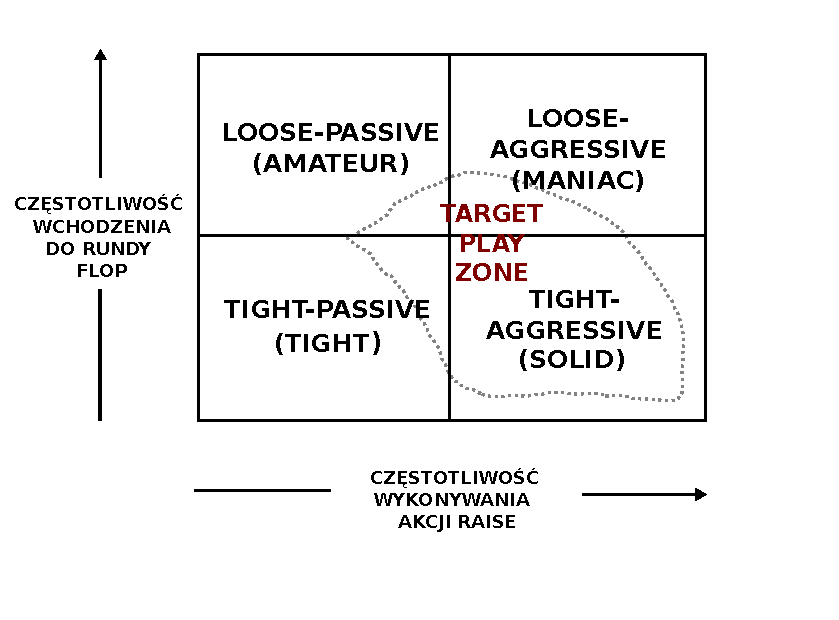
\includegraphics[width=0.5\textwidth]{./img/class.pdf}
           \caption{Podział graczy w grze Poker Texas Hold'em \cite{class}.}
\end{figure}


Jak wynika z powyższych kategorii, gra Poker Texas Hold'em zawiera wiele elementów niezwiązanych z
losowością, gdzie obserwacje i dobieranie odpowiedniej strategi do typu gracza pełni kluczową
funkcję. Korzystając z tych informacji, będzie można określić poziom zaawansowania i styl gry
utworzonych modeli,
które są opisane w rozdziale 4.

\section{Uczenie przez wzmacnianie}

Jest wiele sposobów na stworzenie sztucznych inteligencji w grach. Między innymi można użyć technik 
uczenia
nadzorowanego pod warunkiem, jeśli przygotuje się odpowiednie zbiory danych. W pracy jednak
zdecydowano się na stworzenie modelu, korzystając z uczenia przez wzmacnianie, czyli rozwiązania gdzie
AI nie potrzebuje wstępnej bazy uczącej. Wynika to z faktu, że jest mało publicznych zapisów
gry Poker Texas Hold'em z profesjonalnymi graczami, które mogłyby posłużyć jako zbiory danych.


Algorytmy należące do
wybranego działu powinny być w stanie polepszać swoje wyniki na podstawie interakcji ze
środowiskiem bez korzystania z zewnętrznych materiałów.  
Wiele istniejących metod należących do wybranej techniki zakłada, że środowisko można opisać
przez model
matematyczny
MDP (\emph{Markov Decision Process}). 
Określa ona sekwencyjnie podejmowane decyzje wraz z uzyskiwaną nagrodą od środowiska \cite{mdp}. W każdym z nowych
stanów, w
jakich znajduje się agent (AI), wykonuje on pojedynczą akcję \emph{a}, 
zyskując od środowiska informacje o nowym stanie \emph{s}
oraz nagrodzie \emph{r}. Elementem wyjściowym zasady powinien być
zbiór strategii w postaci modelu, rys. 2.2.


\begin{figure}[th!]
            \center
           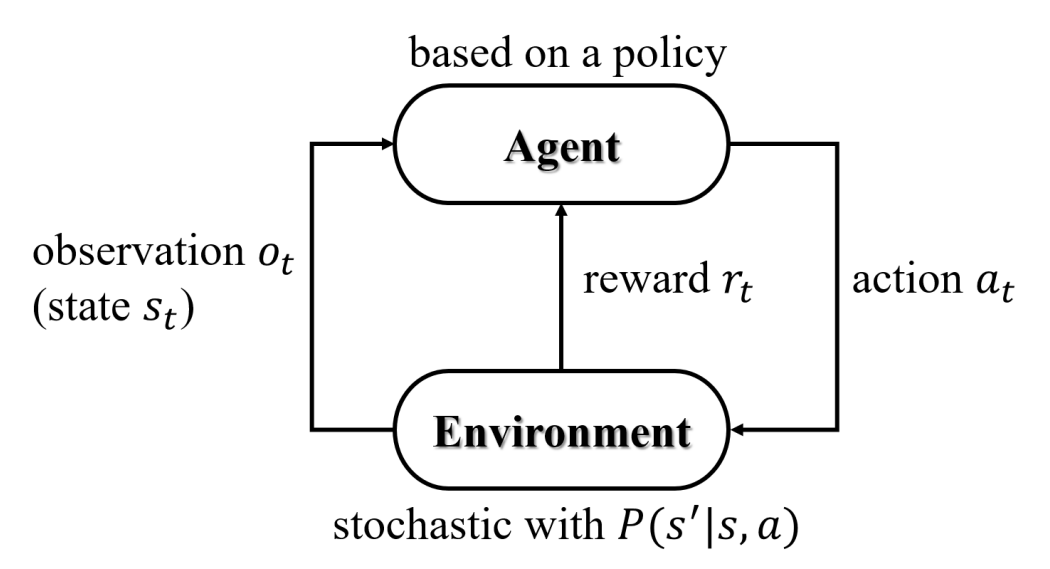
\includegraphics[width=0.5\textwidth]{./img/MDP.png}
           \caption{Schemat modelu matematycznego MDP \cite{mdp}.}
\end{figure}


MDP może opisywać jedynie środowiska z pełnym zakresem informacji, w przypadku algorytmu będącego
tematem pracy, głównym zadaniem jest rozwiązanie środowiska z niepełnym zestawem danych. Wtedy 
należy rozpatrywać zasadę POMDP (\emph{Partially Observable Markov Decision Process}) \cite{mdp}.


W przeciwieństwie do poprzedniego modelu w tym przypadku agent nie zna aktualnego stanu, w którym
się znajduje \cite{mdp}. Przez takie okoliczności musi połączyć zależnością wykonywane akcie i
obserwacje, a nie stany. Większość gier karcianych można zakwalifikować do tego typu problemów
\cite{mdp}.

\section{Teoria Gier}

Aby zrozumieć działanie algorytmów CFR, Deep CFR, MCCFR itd. należy zapoznać się
z podstawami działu matematyki o nazwie Teoria Gier. Bada on optymalne zachowanie w środowiskach, gdzie
występuje konflikt \cite{rn}. W przypadku gry Poker Texas
Hold'em zostały opisane terminy Równowaga Nasha oraz
postać ekstensywna. Są one obowiązkowe do zrozumienia algorytmu Deep CFR.

\subsubsection{Gra w postaci ekstensywnej}

Gry w
formie ekstensywnej można przedstawić jako drzewo decyzyjne, gdzie każdy węzeł rozgałęzia się na
możliwe akcje oraz identyfikuje aktualny stan gracza przez zestaw informacji.
Stany końcowe drzewa określają zysk lub stratę nagrody wybranego gracza \cite{DCFR}.
Jest to sposób
na uproszczenie opisu gry, gdzie ruchy są wykonywane nierównocześnie.

Na rys. 2.4 przedstawiono przykład gry 'Papier-Kamień-Nożyce' w formie ekstensywnej, gdzie gracze P1 i
P2 eksplorują 3 akcje w swoich węzłach. 
Każdy z nich uzyskuje wyniki danych ścieżek oraz zapamiętuje dotychczasową historię, co może zostać potem
wykorzystane do znalezienia najbardziej opłacalnych strategii.

\begin{figure}[th!]
            \center
           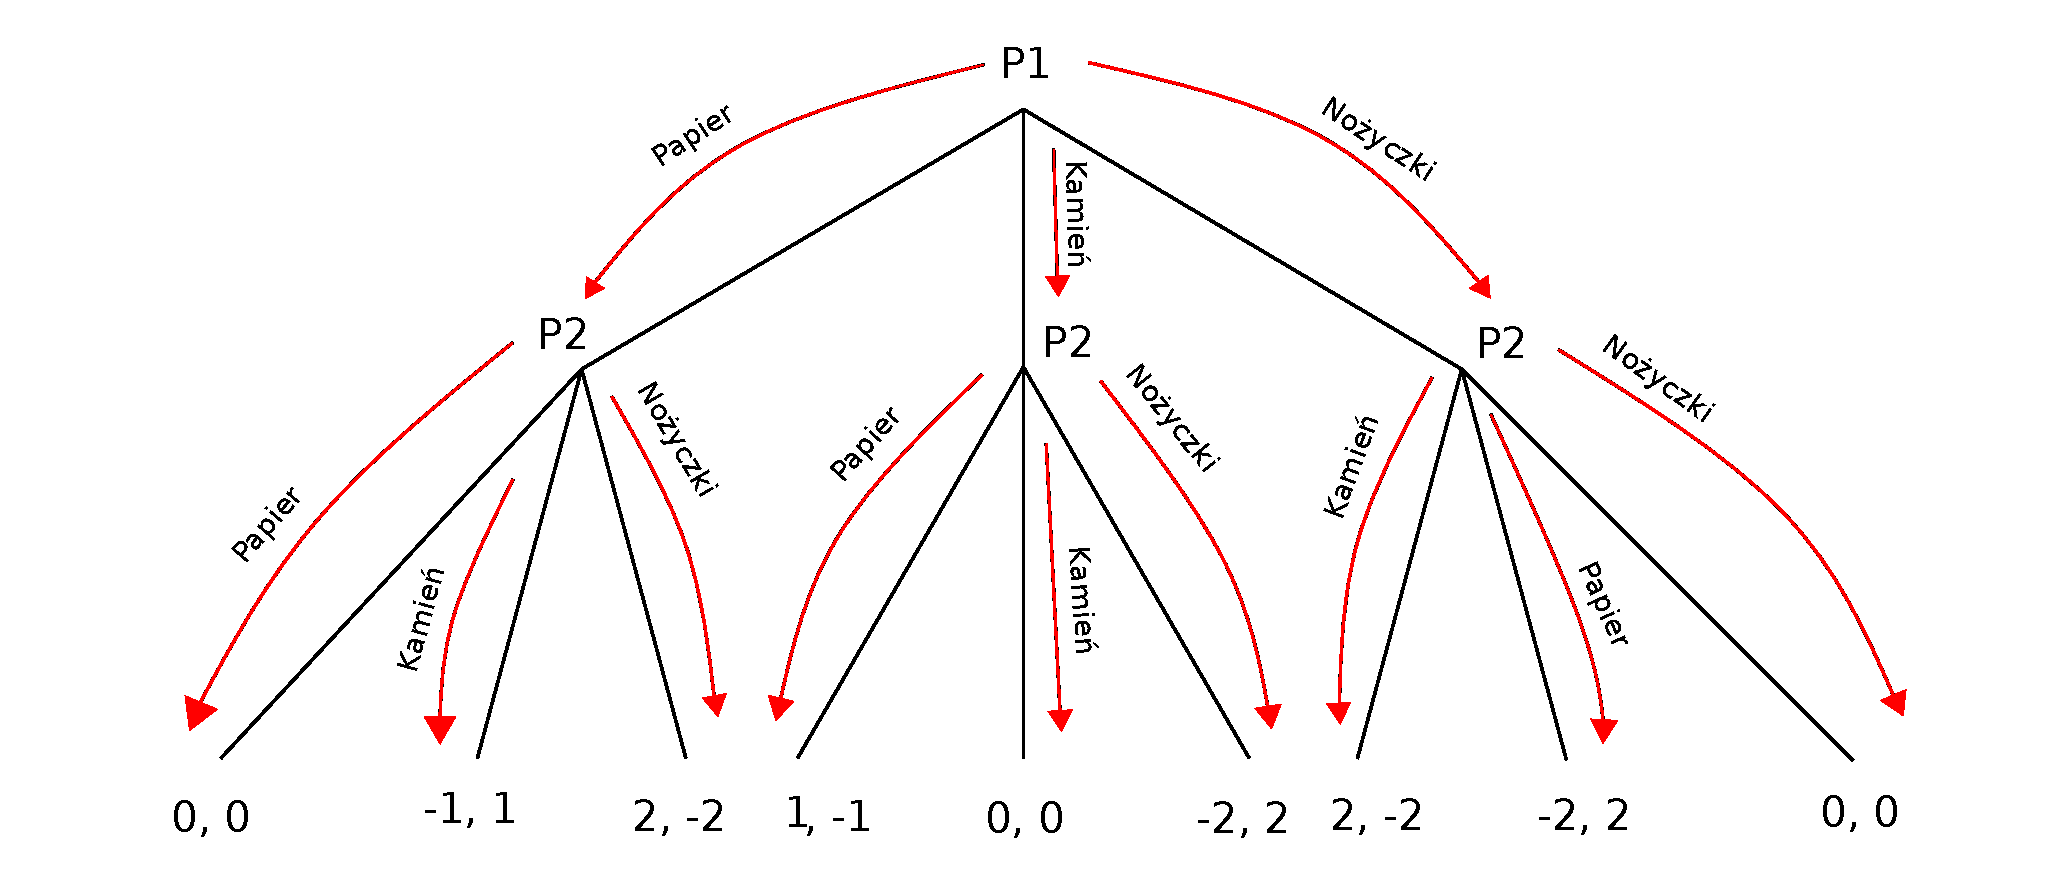
\includegraphics[width=0.9\textwidth]{./img/drawing1.pdf}
           \caption{Opis gry w postaci ekstensywnej.}
\end{figure}

\vspace{5cm}
\subsubsection{Równowaga Nasha}

W grach to twierdzenie określa perfekcyjny stan wyboru akcji, gdzie wszyscy gracze wykorzystują najlepszy
zestaw strategii, którego zmiana przyniesie tylko straty. Oznacza to, że nie jest możliwa
zmiana ruchów na lepsze oraz zwiększenie uzyskanej nagrody przy spełnieniu tej zasady \cite{rn}. 

Dobrym przykładem prezentującym taki stan jest "Dylemat Więźnia" \cite{rn}. Takie środowisko zawiera 
dwóch przestępców, którzy są przesłuchiwani w odseparowanych pomieszczeniach co oznacza, że każdy z
nich ma ograniczony zestaw informacji. Mają oni dwie
opcje, przyznać się do zarzutów lub tego nie robić. Każda z kombinacji akcji jest
zaprezentowana w tab. 2.2, gdzie wartości określają lata spędzone w więzieniu po danym ruchu.
Posługując się Równowagą Nasha, można stwierdzić, że najlepszą opcją dla
obu uczestników będzie przyznawanie się za każdym razem \cite{rn}. Wynika to z faktu, że 
uczestnicy wtedy nie ryzykują.  

Głównym
zadaniem większości algorytmów gier karcianych bazujących na metodzie CFR jest znalezienie
takiego stanu. Deep CFR odkrywa zbiory strategii, które są bliskie Równowadze
Nasha w grach karcianych \cite{DCFR}.

\vspace{1cm}
\begin{table}[h!]
   \centering
\caption{Wyniki akcji środowiska "Dylemat więźnia".}
\begin{tabular}{|c|c|c|}
   \hline
   & \makecell{ więźnia A \\ się przyznaje} & \makecell{więzień A \\ kłamie} \\ 
   \hline
   \makecell{więźnia B \\ się przyznaje} & \diagbox[innerwidth=3cm]{1}{1} & \diagbox[innerwidth=3cm]{0.5}{5} \\
   \hline
   \makecell{więzień B \\ kłamie} & \diagbox[innerwidth=3cm]{5}{0.5} & \diagbox[innerwidth=3cm]{0}{0} \\
   \hline
\end{tabular}

\end{table}



\section{Historia modeli Texas Hold'em Poker}

Bazując na Teorii Gier oraz innych twierdzeniach powstało wiele rozwiązań różnych wersji gry Poker.
Pierwsze dokumenty naukowe omawiały bardzo proste
środowiska rozwiązaywane przez algorytmy jak CFR \cite{DCFR}.


Dopiero w 2015 roku utworzono znaną sztuczną inteligencję $"\text{Cepheus}"$ rozwiązującą problem
HULH \cite{cepheus}. Było to pierwsze takie osiągnięcie w historii. Kolejnym etapem były prace nad
algorytmami mogącym rozwiązać problem gry HUNH (\emph{Heads Up No-limit Texas Hold'em}).
Pierwszy powstały model w 2017 roku nazwano "DeepStack" \cite{ds}. Mieszał on sieci neuronowe z 
technikami algorytmu CFR. W podobnym czasie utworzono kolejne, bardziej zaawansowane AI,
Libratus \cite{libratus}. W 2019 roku pierwszy raz udało się rozwiązać 
problem gry HUNH składającej sie z 6 graczy. Zbudowano model o nazwie "Pluribus", który był
pierwszym AI
rozwiązującym standardową wersję pokera \cite{Pluribus}.


Pomimo takich osiągnięć tworzone modele do 2019 potrafiły grać tylko
w środowiskach 
składających się maksymalnie z 2 osób typu zero-sum \cite{libratus} \cite{cepheus} \cite{ds}.  
Wynika to z poziomu skomplikowania gier częściowo-obserwowalnych.
Sposoby na jego rozwiązanie zaczęły powstawać od niedawna, a pierwsze
dwa duże osiągnięcia w grze HUNH miały miejsce dopiero w 2017 roku.


\subsubsection{Cepheus}

AI powstałe w celu wygrywania w grach HULH. Był to pierwszy model rozwiązujący dużą wersję gry Texas
Poker Hold'em w historii \cite{cepheus}.  Wykorzystał on nowszą wersję techniki CFR, którą nazwano CFR+
\cite{cepheus}. W wyniku dwóch miesięcy nauki i testów nowa metoda zbiegała się znacznie szybciej do
Równowagi Nasha niż bazowy CFR \cite{cepheus}. Powstały model jest udostępniony publiczne, każdy
może go przetestować.    

\subsubsection{DeepStack}

Model DeepStack rozwiązał HUNH przez połączenie metody CFR, sieci neuronowych wraz z dodatkowymi
elementami. W rezultacie AI zaczęło osiągać bardzo dobre wyniki.
Przetestowano go na 33 profesjonalnych graczach w wielu iteracjach gry. Model w większości
przypadków wygrał \cite{ds}. Była to pierwsza wygrana AI z człowiekiem w normalnej 
wersji gry Poker Texas Hold'em z taką częstotliwością.

\subsubsection{Libratus}

Sztuczna inteligencja, która jest wykorzystywana w grach HUNH. Jak wynika z
testów wygrywa znacznie częściej niż DeepStack z profesjonalnymi graczami \cite{libratus}.
Przetestowano go z mistrzami gry, Dong Kim, Dan McAulay, Jimmy Chou 
i Jason Les \cite{libratus}. AI wygrało z nimi, z ogromną przewagą.


\section{Counterfactual Regret Minimization}

\subsection{Regret Matching}

Jest to nieodłączna metoda uczenia AI w grach karcianych. Polega ona na liczeniu najlepszej 
strategii pod warunkiem, że znany jest wektor żalu (\emph{regrets}) w węźle \cite{CFR}.
Taki wektor opisuje się jako tablicę wag o długości równej liczbie możliwych akcji gracza. Każda z 
tych wag opisuje, jak dużym błędem będzie niewykonania danego ruchu.


Poniżej przedstawiono wzór wynikający z tej metody, gdzie  
$R^{t}(a)$ jest omawianym wektorem \cite{CFR}. 
Następnie, aby uzyskać nową strategię, usuwa się wartości ujemne, czyli takie, których gracz nie
żałował (formuła nr 2.2).
Potem sprawdzana się, czy ich suma jest większa od zera w celu wybrania odpowiedniego wzoru, formuła
2.1.
W zależności od tego warunku otrzymuje się określony rozkład prawdopodobieństwa wykonania każdej z
akcji.


\begin{equation}
p^{t}_{i}\left( a \right) = \left\{ \begin{array}{ll}
      \frac{R^{T, \text{+}}\left(a\right)}{ \Sigma_{a' \in A} R^{T,\text{+}}\left(a'\right)} &
      \mbox{if $\Sigma_{a' \in A} R^{T,\text{+}}\left(a'\right) >
      0$};\\
      \frac{1}{|A|} & \mbox{$otherwise$}.\end{array} \right. \ 
\end{equation}

\vspace{1cm}
\begin{equation}
   R^{t,\text{+}}(a) = max(R^t(a),0)
\end{equation}


Proces ten jest powtarzany wielokrotnie, tak, aby przy każdej iteracji rozkłady prawdopodobieństwa
ruchów były stopniowo
poprawiane.

W przypadku algorytmu Deep CFR zachodzi modyfikacja formuły nr 2.1. Strategia jest liczona na
dodatnich wartościach żalu podzielonego przez  prawdopodobieństwo dostania się do 
tego stanu $D^{T} (I, a)$ \cite{DCFR}.
Jeśli suma jest ujemna, to zostaje wybrana akcja z najwyższą wartością $D^{T}(I, a)$ \cite{DCFR}.



\begin{equation}
\sigma^{t+1}_{i}\left(I, a \right) = \left\{ \begin{array}{ll}
      \frac{D^{T, \text{+}}\left(a\right)}{ \Sigma_{a' \in A} D^{T,\text{+}}\left(a'\right)} &
      \mbox{if $\Sigma_{a' \in A} D^{T,\text{+}}\left(a'\right) >
      0$};\\
      \text{argmax}(D^{T} (I, a)) & \mbox{$otherwise$}.\end{array} \right. \ 
\end{equation}



\subsection{Counterfactual Regret}

Algorytm CFR do znanych wcześniej metod dodał termin 'Immediate Counterfactual Regret' oznaczany przez $R^{T}_{i,
imm} (I)$, 
czyli żal przydzielony do węzła I.
Do obliczenia takiego parametru została zdefiniowana wartość "counterfactual utility" $u_{i}(\sigma,
I)$. Oznacza ona przewidywą opłacalność stanu I gdzie wszyscy gracze używają strategi
$\sigma$ \cite{CFR}. Dodatkowo $\pi^{\sigma} (h, h')$ oznacza prawdopodobieństwo dostania się z historii h do 
nowego stanu h' przy strategii $\sigma$ \cite{CFR}.

\begin{equation}
   u_{i} (\sigma, I) = \frac{\sum_{h \in I, h' \in Z} \pi^{\sigma}_{-i} (h) \pi^{\sigma} (h,
   h') u_{i}(h')}{\pi_{-i}^{\sigma}(I)}
\end{equation}

Na podstawie równania 2.5 można wyliczyć końcową wartość żalu w algorytmie CFR.

\begin{equation}
   R^{T}_{i,\text{imm}} (I, a) = \frac{1}{T} \sum^{T}_{t=1} \pi^{\sigma^{t}}_{-i} (I)
   (u_{i}(\sigma^{t}|_{I \rightarrow a}, I) - u_{i}(\sigma^{t}, I))
\end{equation}


Powyższe 2 równania można doprowadzić do formuły nr 2.6. Wartość $\pi^{\sigma} (h,h')$ została
zastąpiona przez liczbę 1, ponieważ
CFR zakłada, że dla $u_{i}(\sigma^{t}|_{I \rightarrow a}, I)$, gracz wykonuje zawsze akcję \emph{a} 
z całkowitą pewnością \cite{CFR}.



\begin{equation}
   R^{T}_{i,\text{imm}} (I, a) = \frac{1}{T} \sum^{T}_{t=1}
   \pi_{-i}^{\sigma}(h)\sum_{h \in I, h' \in Z}(1*u_{i}(h') - \pi^{\sigma}(h,h')u_{i}(h'))
\end{equation}


\vspace{0.5cm}
Po uzyskaniu $R^{T}_{i,\text{imm}} (I, a)$ można wykorzystać metodę "Regret Matchning" i
zaktualizować strategie.
Poniżej przedstawiono przykład obliczeń pojedyńczego węzła P2 oraz wyniki 
dla gry "Papier-Kamień-Nożyce" przy ustawionych
nagrodach i karach w stanach końcowych jak na rys. 2.4, 2.5, 2.6.

\begin{center}
$$
   \pi^{\sigma}(h,h')u_{i}(h') =  (\frac{1}{3} \cdot 0) + (\frac{1}{3} \cdot -1) +
   (\frac{1}{3} \cdot 2) = \frac{1}{3}
$$

$$
T*R^{T}_{i,\text{imm}} (I, a) =
((0-\frac{1}{3}), (-1-\frac{1}{3}), (2-\frac{1}{3})) \cdot \frac{1}{3}= (-\frac{1}{9},
-\frac{4}{9}, \frac{5}{9}) 
$$

$$
\sigma^{t+1}_{i}\left(I, a \right) = (0, 0, 1)
$$
\end{center}
\vspace{0.5cm}


\begin{figure}[th!]
            \center
           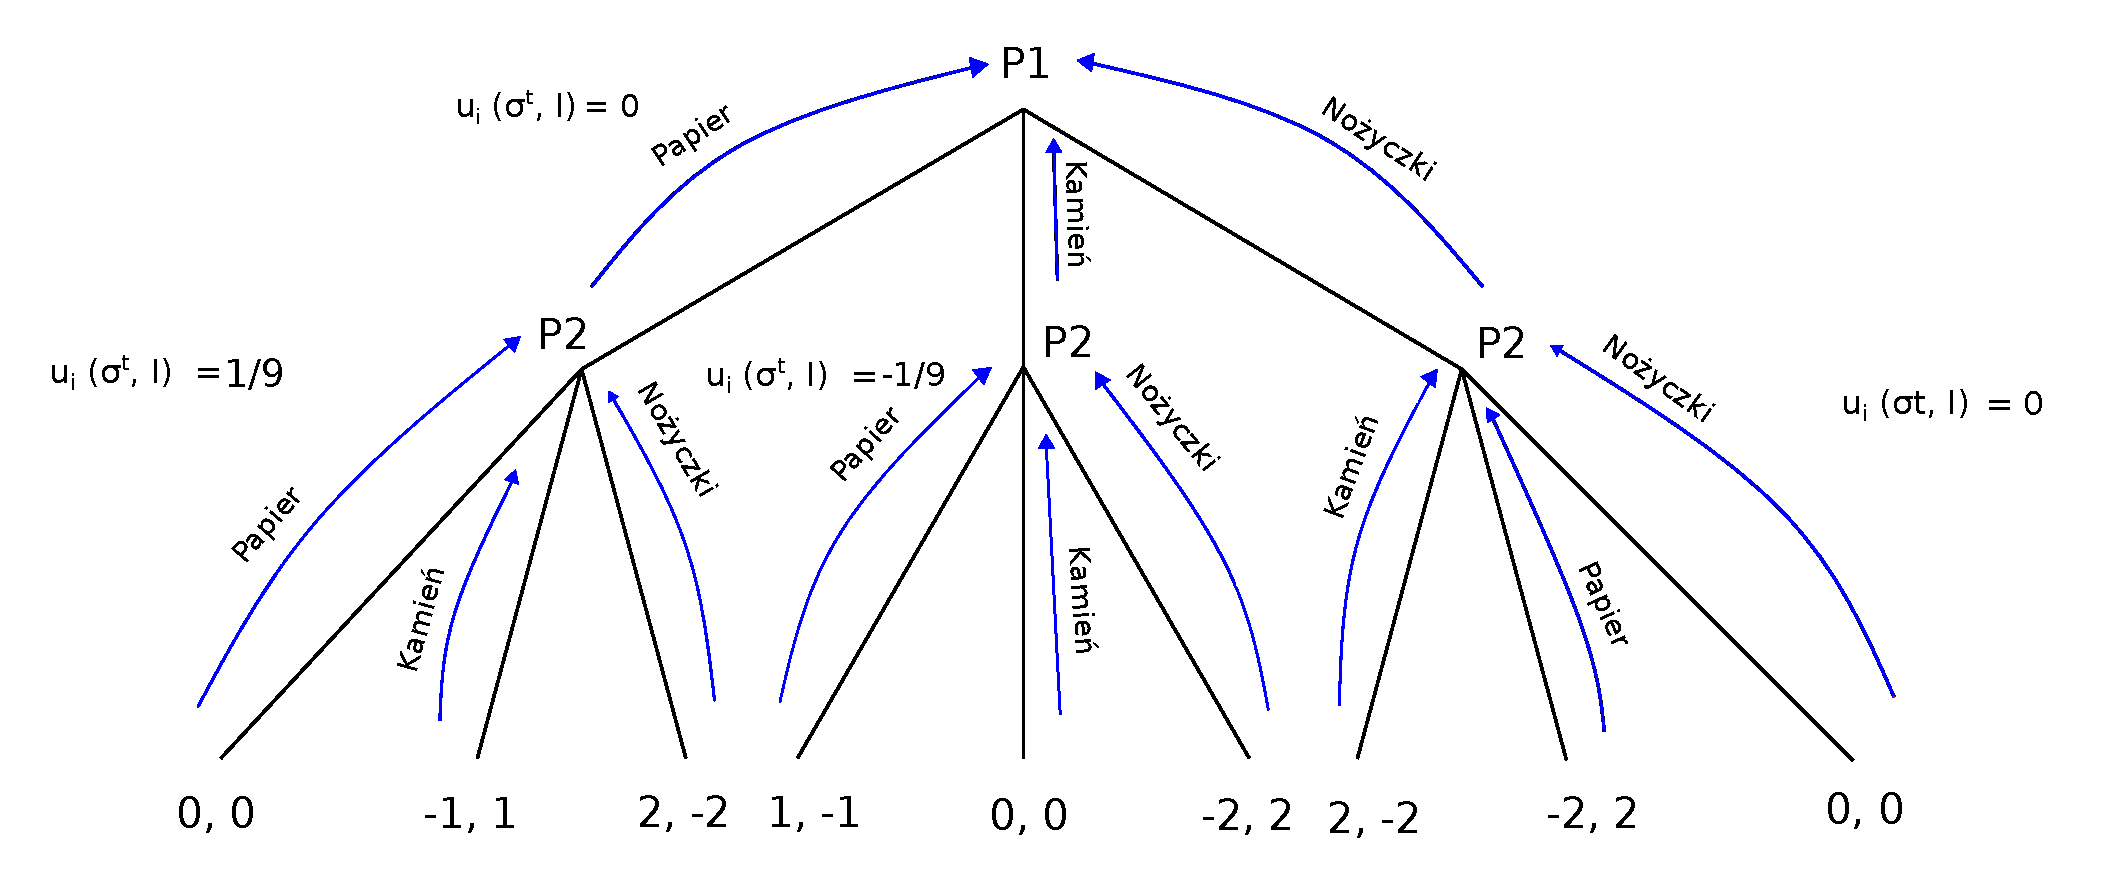
\includegraphics[width=1\textwidth]{./img/drawing2.pdf}
           \caption{Przykład obliczonych wartości 'counterfactual utility'.}
\end{figure}

Na podstawie rys. 2.4 widać, że gracz P2 będzie miał stan o najwyższej wartości "counterfactual utility" w węźle $u_{i}
(\sigma^{t}, I)=\frac{1}{9}$, a najniższej dla $u_{i}(\sigma^{t}, I)=-\frac{1}{9}$.


\begin{figure}[th!]
            \center
           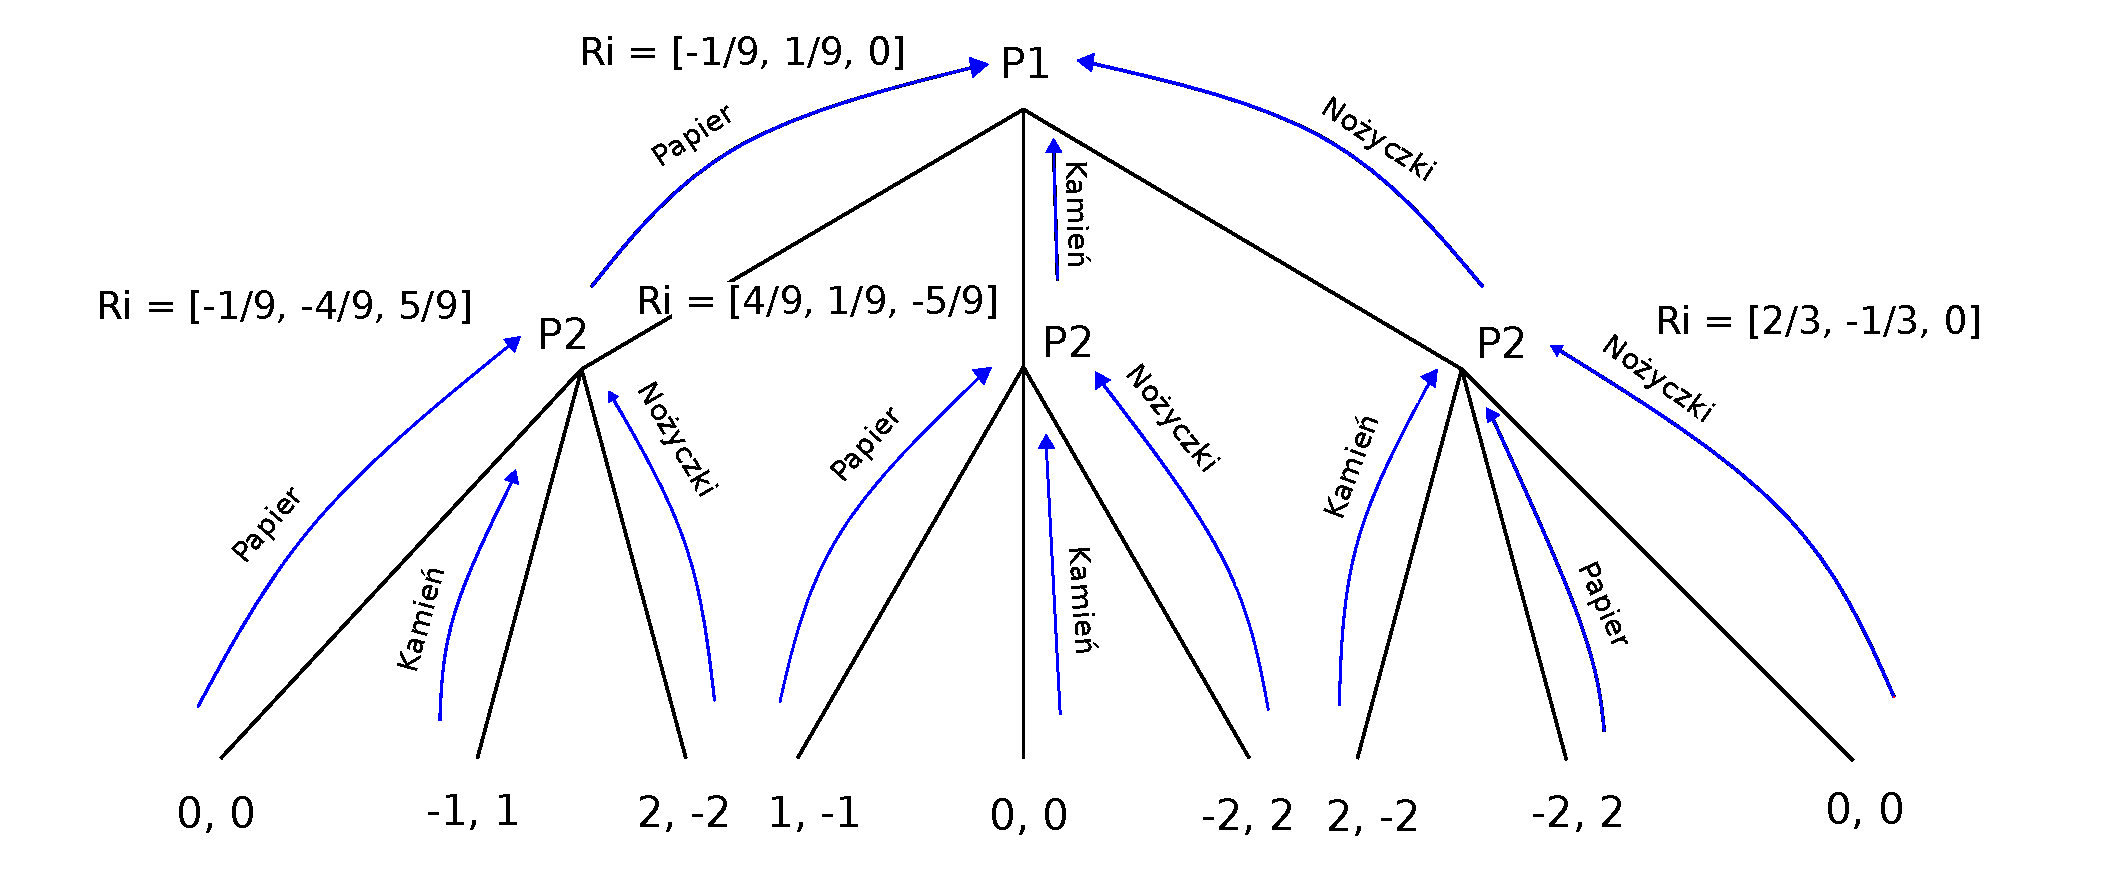
\includegraphics[width=1\textwidth]{./img/drawing3.pdf}
           \caption{Przykład obliczonych wartości 'Immediate Counterfactual Regret'.}
\end{figure}

\vspace{0.5cm}
\vspace{10cm}

Powyżej zaprezentowano wektory $R^{T}_{i,\text{imm}} (I, a)$.
Gracz P1 grając, najbardziej będze żałował nie wykonania akcji \emph{Kamień}, a najmniej
\emph{Papier}.

\vspace{0.5cm}
\begin{figure}[th!]
            \center
           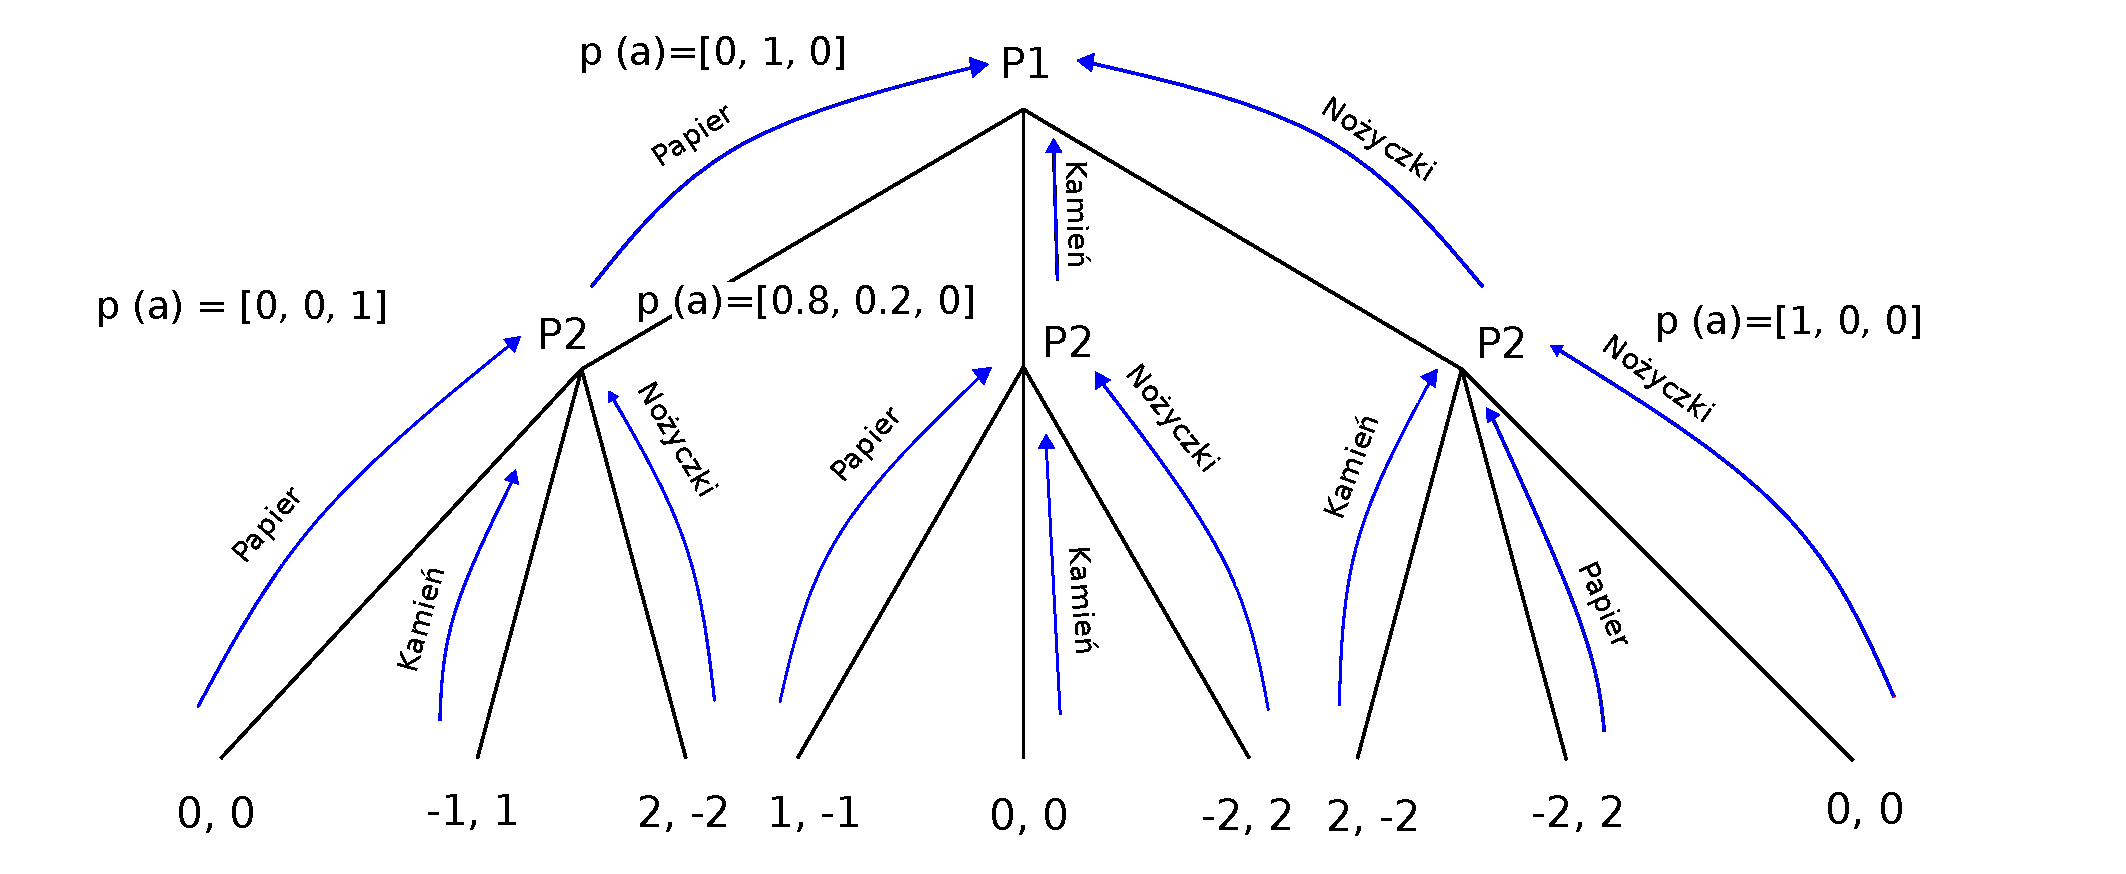
\includegraphics[width=1\textwidth]{./img/drawing4.pdf}
           \caption{Przykład obliczonych strategii.}
\end{figure}
 
Rys. 2.6 przedstawia wektory określające jakimi rozkładami akcji powinni się kierować gracze, aby
osiągnąć najlepsze wyniki. Są to wektory wyliczone po pierwszej iteracji, w praktyce eksploracja
drzewa i powyższe obliczenia są powtarzane wielokrotnie. Końcowym etapem algorytmu CFR jest
policzenie średniej strategii, która ma reprezentować Równowagę Nasha \cite{CFR}.





\section{Monte Carlo Conterfactual Regret Minimization}

Algorytm CFR eksploruje całe drzewa decyzyjnego w jednej iteracji, co tworzy wymagania na
dużą moc obliczeniową i długi czas uczenia. Dla małych gier takie rozwiązanie jest akceptowalne, ale w przypadku 
większych środowisk jest nieefektywne.
Spowodowało to powstanie nowszej wersji algorytmu CFR, MCCFR (\emph{Monte Carlo Conterfactual Regret
Minimization}) , 
który w każdą iterację eksploruje tylko część drzewa \cite{mccfr}.

Metodę można podzielić na dwie odmiany, Outcome-Sampling oraz External-Sampling \cite{mccfr}.

W pracy został przedstawiony sposób MCCFR ES (\emph{Monte Carlo Conterfactual Regret
Minimization External Sampling}), ponieważ taki jest zaimplementowany w algorytmie
Deep CFR.
MCCFR ES przed eksploracją drzewa wybiera kolejno spośród graczy jednego uczestnika, którego 
oznacza
się jako "traverser" \cite{DCFR}.
Eksploruje on wszystkie odpowiedzi ze swoich akcji w danym węźle. W międzyczasie inni
uczestnicy wykonują pojedynczy ruch na podstawie swojej najlepszej strategii \cite{mccfr}.  


Na rys. 2.7 przedstawiono przykład części drzewa HULH, 
gdzie gracz P2
został wybrany jako "traverser". 
Jak można zauważyć, tylko jego węzły rozgałęziają się na wszystkie możliwe ścieżki. 
Dodatkowo w drodze powrotnej obliczono $u_{i} (\sigma, I)$ dla wszystkich
stanów używając wzoru 
2.5.


\begin{figure}[!ht]
  \centering
  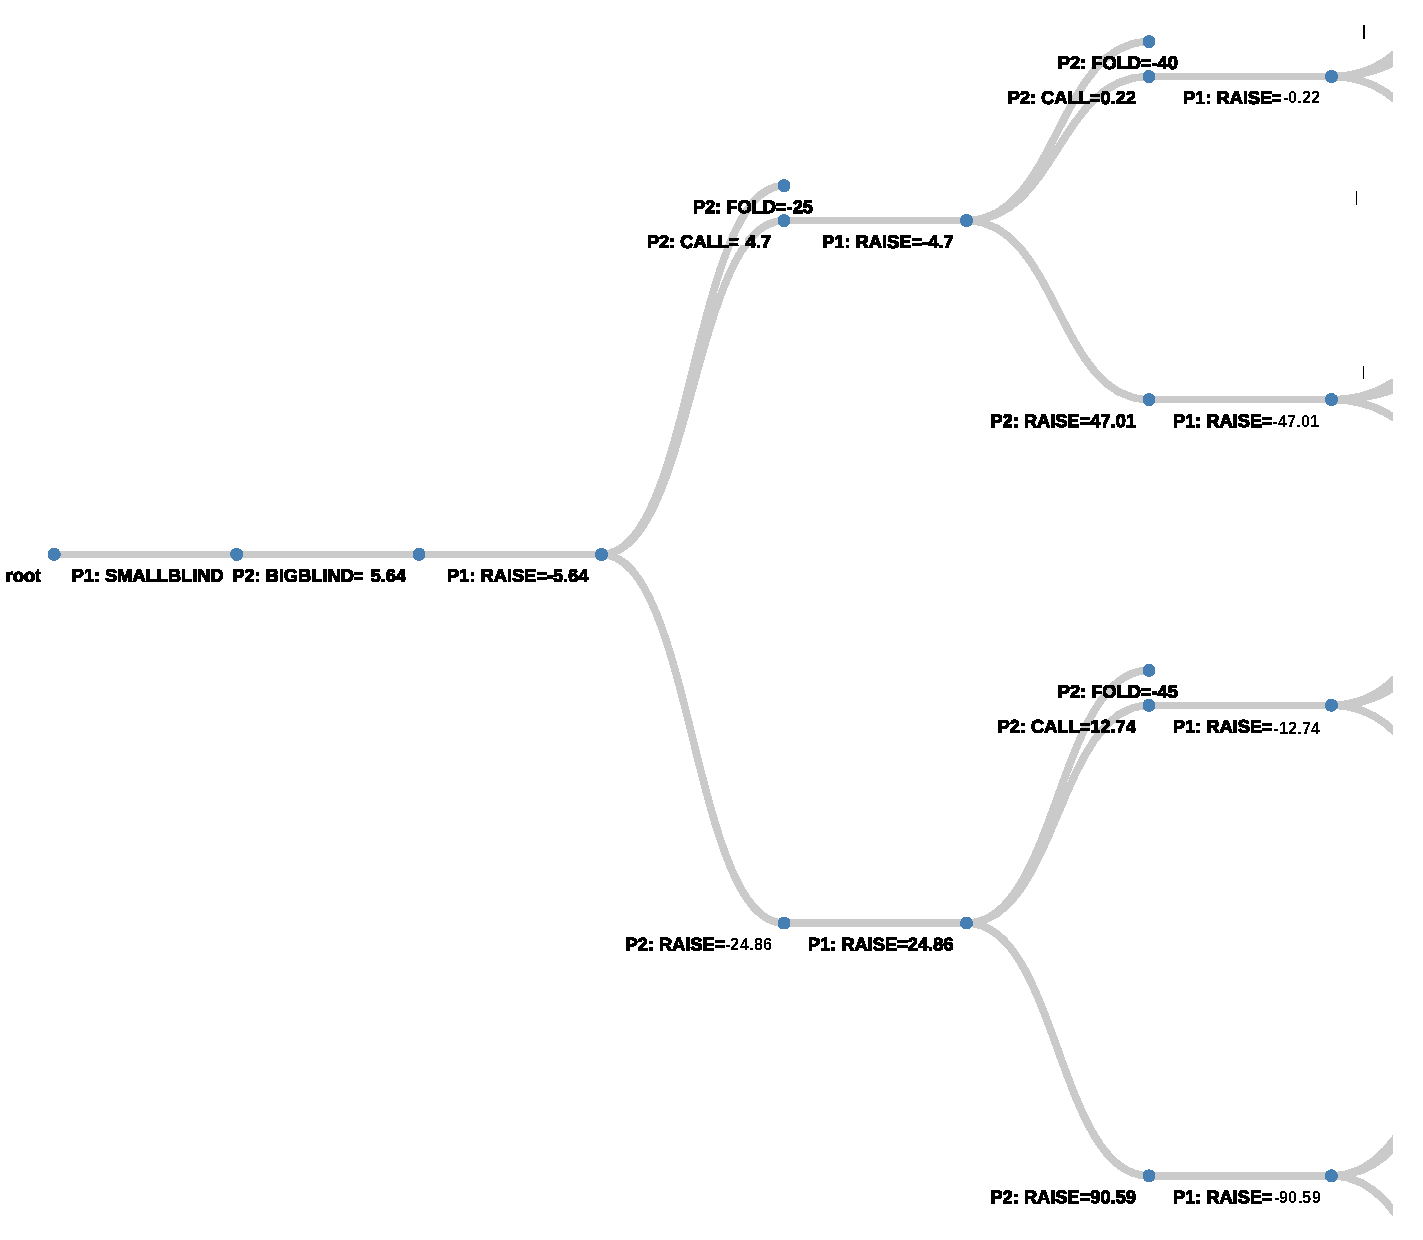
\includegraphics[width=1\textwidth]{./img/tree.pdf}
  \caption{Część drzewa decyzyjnego MCCFR ES z graczem P2 jako "traverser".}
\end{figure}


\vspace{5cm}
Jest to przykład z jednej eksploracji gry, w praktyce powtarza się ten proces wielokrotnie, 
uzyskując różne wersje drzew.


Mając takie wyniki, można przystąpić do liczenia $R_{i,imm}^{T} (I)$ oraz poprawiania 
wartości przez "Regret Matching". MCCFR ES spełnia swoją funkcję, ale wymaga wielu iteracji, aby
uzyskać dobre wyniki. Z tego powodu w dalszym rozdziale zostanie przedstawiona metoda Deep CFR,
która przyspiesza proces uczenia przez użycie sieci neuronowych.

\section{Deep CFR}


Algorytm Deep CFR  opisany w \cite{DCFR} rozwija podstawową wersję metody CFR o sieci neuronowe.
Taka modyfikacja była wymagana, aby utworzyć AI, które może rozwiązać duże gry
jak HULH znacznie szybciej. Liczy on wektory w drzewie decyzyjnym
przez algorytm MCCFR ES. Dodatkowo Deep CFR okazał się lepszy niż 
popularny algorytm NFSP z 2016 roku \cite{DCFR}.

Deep CFR wykorzystuje sieci neuronowe do przewidzenia wartości $D^{T}$(I, a) w podobnych
obserwacjach, potem na
podstawie predykcji liczy strategię ze wzoru nr 2.3.   
Następnie liczona jest zaktualizowana wersja wektora żalu, formuła nr 2.5.
Obliczone wyniki są dodawane do buforów  $($B_{1}$, $B_{2}$) \in B_{p}$, a strategia do zbioru $B_{s}$.


Po wielu iteracjach
rozpoczyna się nauka sieci z zebranej bazy. Poniżej przedstawiono dokładny opis Deep CFR.
\vspace{1cm}

\begin{algorithm}[H]
\SetKwInput{KwInput}{Wejście}                % Set the Input
\SetKwInput{KwOutput}{Wyjście}              % set the Output
\DontPrintSemicolon
  
\KwInput{$B_{p}$, $B_{s}$, $\theta_{s}$, $\theta_{p}$, $P$, $N$, $K$}
\KwOutput{$\theta_{s}$}
\For{n \textbf{in} $N$}{
   $h$, $t$ \leftarrow \text{Nowa gra}\\
   \For{$p$ \textbf{in} $P$}{
      \For{$k$ \textbf{in} $K$}{
         MCCFRES($\theta_{p}$, $\theta_{p-1}$, $p$, $t$, $h$, $B_{p}$, $B_{s}$)\\
      }
      $\theta_{p}$ \leftarrow \text{TRAIN($B_{p}$, $\theta_{p}$, $t$)} \Comment{loss:
         $\frac{1}{N_{batch}}$
      $\sum(y_{i}-\widehat{y_{i}})^2$$\cdot$$t_{i}$}\\
   }
}
$\theta_{s}$ \leftarrow \text{TRAIN($B_{s}$, $\theta_{s}$, $t$)} \Comment{loss:  $\frac{1}{N_{batch}}$$\sum(y_{i} -\widehat{y_{i}})^2$$\cdot$t_{i}$}\\
\textbf{return} $\theta_{s}$
 \caption{Deep CFR}
\end{algorithm}

\vspace{1cm}
Algorytm na wejściu dostaje argumenty przystosowane do gry 2-osobowej.
Pierwszymi elementami są bufory graczy ($B_{1}$, $B_{2}$) oraz kontener na 
strategie $B_{s}$.
Dodatkowo metoda potrzebuje listę uczestników \emph{P}, z których będzie wybierany cyklicznie gracz
eksplorujący drzewo decyzyjne.
Ostatnimi argumentami są iteracje gry \emph{N} oraz liczba cykli \emph{K} metody MCCFR ES.


Podsumowując należy ustawić trzy pętle wraz z nową rundą, uzyskując początkową historię oraz
krok gry t. Kolejnym etapem jest
wykonanie funkcji \emph{MCCFRES}. Przyjmuje ona na wejściu sieci neuronowe obu graczy, 
listę uczestników p,
numer kroku t, historię rundy h oraz bufory. Po k 
powtórzeniach następuje uczenie sieci neuronowej wybranego wcześniej gracza eksplorującego drzewo. 

Model używa 
zmodyfikowanej wersji funkcji MSE (\emph{Mean Square Error}) do liczenia błędu predykcji. Każdy wynik $(y_{i} - \hat{y_{i}})^2$
mnożony jest przez krok $t_{i}$ w, którym uzyskano $y_{i}$ \cite{DCFR}.
Dodatkowo jak wynika z badań, algorytm osiąga lepsze wyniki
jeśli
sieci neuronowe są trenowane od początku \cite{DCFR}. Dlatego należy przed funkcją \emph{TRAIN}
wyczyścić model.

Po wszystkich powtórzeniach i zebraniu całej bazy bufora $B_{s}$, rozpoczyna się trenowanie sieci 
neuronowej $\theta_{s}$ w ten sam sposób jak inne modele. Elementem wyjściowym Deep CFR jest sieć 
$\theta_{s}$.


\vspace{1cm}
\begin{algorithm}[H]
\SetKwInput{KwInput}{Wejście}                % Set the Input
\DontPrintSemicolon
\SetKwFunction{FMain}{MCCFRES}
\SetKwProg{Fn}{Function}{:}{}
  
\Fn{\FMain{$\theta_{p}$, $\theta_{p-1}$, $p$, $t$, $h$, $B_{p}$, $B_{s}$}}{
   $t_{r}$ \leftarrow h \Comment{sprawdzenie czyja jest aktualnie tura}\\

   \uIf{$h$ jest stanem końcowym Z}{
      \textbf{return} $u_{p} (h)$
   }
   \uElseIf{$p$ = $t_{r}$}{
      $\hat{D}(I)$ \leftarrow \text{utworzenie wektora $\hat{D}(I)$ z sieci $\theta_{p}$}\\
      $\sigma (I)$ \leftarrow \text{obliczenie strategi $\sigma_{t_{r}} (I)$, kożystając z $\hat{D}(I)$ i
         wzoru 1.1}\\

      \For{a \textbf{in} A(h)}{
         $u_{t_{r}}$(ha) \leftarrow \FMain{$\theta_{p}$, $\theta_{p-1}$, $p$, $t+1$, $h+a$, $B_{p}$,$B_{s}$}\\
          
      }
      $u_{r_{r}}(\sigma, I)$ \leftarrow $\sum (u_{t_{r}}(ha) \cdot \sigma(I))$\\
      $R^{T}_{t_{r}}$(I) \leftarrow ($u_{t_{r}}(ha) - u_{t_{r}}(\sigma, I)$)\\
      $B_{t_{r}}$ \leftarrow \text{dodanie próbki  } $[R^{T}_{t_{r}}$(I), h, t]$ \text{ do
      bufora}\\

   }
   \Else{
      $\hat{D}(I)$ \leftarrow \text{utworzenie wektora $\hat{D}(I)$ z sieci $\theta_{p}$}\\
      $\sigma (I)$ \leftarrow \text{obliczenie strategi $\sigma_{p} (I)$, kożystając z $\hat{D}(I)$ i
         wzoru 1.1}\\
      $B_{s}$ \leftarrow \text{dodanie próbki } $[\sigma (I), h, t]$ \text{ do bufora}\\
      a \leftarrow $\sigma (I)$

      \textbf{return} \FMain{$\theta_{p}$, $\theta_{p-1}$, $p$, $t+1$, $h+a$, $B_{p}$,
         $B_{s}$}\\
   }
}
 \caption{Implementacja MCCFRES kożystając z sieci neuronowych}
\end{algorithm}

\vspace{1cm}

Implementacja MCCFR ES przedstawiona powyżej przy zadanych argumentach rozpoczyna się od
sprawdzenia, który gracz rozpoczyna daną turę. Na podstawie tej informacji będzie wykonywana
dalsza część algorytmu.


Pierwszym krokiem jest sprawdzenie, czy stan gry jest końcowym etapem. W przypadku prawdziwego 
warunku zwracana jest wygrana lub przegraną wartość stawki. 
Jeśli powyższy etap jest fałszywy, algorytm sprawdza, czy gracz jest oznaczony jako "traverser".
Wtedy program używając sieci neuronowej gracza,
otrzymuje wektor $\hat{D}(I)$ przez wprowadzenie do modelu informacji o widocznych kartach oraz
dotychczasowej historii gry. Korzystając ze wzoru 2.3, liczy strategie, odczytuje wektor $u_{t_{r}}$ (ha) 
wykonując rekurencję. Ostatnim krokiem jest wyliczenie wektora żalu i dodanie go do bufora.

Jeśli powyższy warunek był fałszywy, gracz liczy nowy rozkład
akcji i dodaje go do zbioru strategii. Następnie korzystając z tej sieci neuronowej i otrzymanej 
dystrybucji wykonuje nową akcję.


\section{Podsumowanie}

Środowiska z niepełnym zestawem informacji i brakiem deterministyczności są trudne do rozwiązania.
Algorytmy tworzące modele
dla takich gier są często skomplikowane i obciążające obliczeniowo. 
Przez takie cechy dopiero od niedawna zaczęły powstają algorytmy, zdolne pokonać ludzi w 
dużych grach karcianych jak "Cepheus", "DeepStack", "Libratus" lub "Pluribus". 
Metody zdolne tworzyć takie AI dalej są rozwijane i aktualizowane z roku na rok.
W taki sposób w 2007 roku powstał CFR, potem MCCFR i po para latach zastąpiono je przez CFR+, aż 
zaczęto wykorzystywać sieci neuronowe w takich algorytmach jak 
Deep CFR będący tematyką pracy. 

Rozdział dokładnie opisał działanie omawianego algorytmu
przez przedstawienie terminów należących do działu matematyki Teoria Gier. Między innymi
 pokazał, że opis środowiska przez drzewa decyzyjnych pozwala na wiele uproszczeń i możliwości
 śledzenia gry. Dodatkowo przedstawiono problem poszukiwania stanu Równowagi Nasha, którego
 znalezienie jest celem większości algorytmów sztucznej inteligencji gier karcianych.

Dobrze zaimplementowany algorytm Deep CFR przy prawidłowej parametryzacji i odpowiednio dużej
liczby iteracji powinien zbiec się do punktu bliskiego takiego stanu. Pomimo tak optymistycznych 
założeń utworzonie AI potrzebuje bardzo długiego czasu nauki do 
znalezienia dobreych strategii gry w HULH i HUNH.


\chapter{Implementacja algorytmu} 

Program Deep CFR został napisany w niniejszej pracy, korzystając z narzędzi,
pozwalających na zredukowanie nadmiarowości kodu oraz na prostą implementację.
W tym rozdziale skupiono się na opisaniu wybranych technologii, parametrów oraz funkcji, 
które znalazły się w implementacji algorytmu.

Bazą do napisanego kodu jest język programowania, Python 3.8. Zawiera on wiele
technologii wspomagających uczenie maszynowe i rozległą społeczność wspierającą jego rozwój.
Poniżej 
wylistowano i opisano główne narzędzia użyte w pracy.

\paragraph{TensorFlow}

Jest to wysokopoziomowe API dostępne dla takich języków jak Python, JavaScript, C++ lub Java
\cite{tensorflow}.
Wykorzystuje je się głównie do zadań głębokiego uczenia maszynowego. Przez swoją prostotę, dostępność 
i dobrą
dokumentację stał się jednym z najpopularniejszych narzędzi wykorzystywanych do tworzenia
sztucznych inteligencji. Dodatkowo od niedawna biblioteki technologi Keras stały się częścią Tensorflow.
Daje to możliwości znacznego
zredukowania kodu przy prostych problemach, które często są rozwiązane przez funkcje w tym module. 


W przypadku niniejszej pracy głównie korzystano z funkcji zawartych w bibliotekach Keras. Wyjątkiem 
są nieliczne wiersze w kodzie gdzie np. było wymagane wykonanie obliczeń na tensorach.

\paragraph{Numpy}

Duża biblioteka do naukowych obliczeń na wielowymiarowych tablicach. Jest nieodłącznym
elementem przy pisaniu programów uczenia maszynowego, zwłaszcza jeśli korzysta się z 
bibliotek Tensorflow. Wynika to z faktu, że wiele funkcji tego API, jako argumenty przyjmuje
typy danych powiązane z Numpy \cite{tensorflow}.



\paragraph{Tqdm}
Małe narzędzie w języku Python pozwalające na wyświetlenie postępu procesów w działającym 
programie.
Przydatne w celach
testowych. W pracy zostało użyte do śledzenia iteracji drzew decyzyjnych 
algorytmu Deep CFR.

\paragraph{TensorBoard}
Moduł należący do API Tensorflow. Wizualizuje postępy uczenia sieci neuronowych oraz ich 
jakość przez przedstawienie odpowiednich wykresów. 


\paragraph{PyPokerEngine}

Biblioteka wspomagająca symulację gry Poker Texas Hold'em wraz z dodatkowymi elementami.
Użyto jej jako podstawę do napisania środowiska HULH.

\section{Implementacja sieci neuronowych}

Algorytm Deep CFR do działania wymaga dwóch typów sieci neuronowych, jedna ma rozpoznawać strategie
$\sigma^{t}$, a
druga przypisana do określonego gracza przewiduje wartości $D_{p}^{t}$. 
Dodatkowo każdy z tych elementów
jest trenowany na podstawie cyklicznie aktualizowanych buforów $B_{s}$ i $B_{p}$. W tym rozdziale zostanie
przedstawiona dokładna implementacja modeli, proces ich uczenia, struktura zbiorów danych oraz
budowa środowiska, z którym jest wykonywana interakcja. W tab. 3.1 i 3.2 zamieszczono podstawowe 
informacje
o parametrach sieci. Dalsza część rozdziału dokładnie opisuje te parametry i dodatkowe elementy, ważne podczas
uczenia modelu.

\vspace{1cm}
\begin{table}[h!]
\centering
\caption{Podstawowe parametry sieci neuronowej $\theta_{s}$.}
\begin{tabular}{|c|c| }
   \hline
   parametr & użyte wartości \\
    \hline
   prędkość uczenia & 0.0001 \\
   \hline
   końcowa funkcja aktywacyjna & \emph{softmax} \\
   \hline
   rozmiar bufora & 600 000 \\
   \hline
   maksymalna liczba iteracji & 5 000 \\
   \hline
   rozmiar \emph{minibatch} &  500\\
   \hline
   parametr \emph{patience} &  40\\
   \hline
\end{tabular}
\end{table}

\begin{table}[h!]
\centering
\caption{Podstawowe parametry sieci neuronowej $\theta_{p}$.}
\begin{tabular}{|c|c| }
   \hline
   parametr & użyte wartości \\
    \hline
   prędkość uczenia & 0.0001 \\
   \hline
   końcowa funkcja aktywacyjna & \emph{linear} \\
   \hline
   rozmiar bufora & 300 000 \\
   \hline
   maksymalna liczba iteracji & 5 000 \\
   \hline
   rozmiar \emph{minibatch} &  500\\
   \hline
   parametr \emph{patience} &  40\\
   \hline
\end{tabular}
\end{table}

\vspace{5cm}
\subsection{Architektura modelu}

W algorytmie zaimplementowano trzy sieci neuronowe $\theta_{1}$, $\theta_{2}$, $\theta_{s}$ o nieskomplikowanej architekturze. Z tego powodu
wykorzystano bibliotekę Keras, która do takich przypadków jest dobrym rozwiązaniem. 
Dodatkowo
założono, że
wszystkie modele będą miały podobną budowę poza ostatnią warstwą z innymi funkcjami
aktywacyjnymi. Wynika to z faktu, że algorytm Deep CFR korzysta z sieci, które dostają dane wejściowe
o tej samej strukturze, ale zwracają $D_{p}^{t}$ lub $\sigma_{p}^{t}$.

Architektura sieci neuronowych składa się z 7 elementów, wejścia, wyjścia, bloku o nazwie
$\emph{Flatten}$ \cite{tensorflow}, 
trzech warstw ukrytych zakończonych normalizacją i wyjściem w postaci wektora o trzech polach.
Początkowo sieci dostają tablicę o wymiarach (3, 52), czyli kolumnę kart ze stołu, z ręki oraz
historię ostatniej rundy gry. Model w dalszych obliczeniach musi
przekształcić takie dane do formy jedno-wymiarowej (None, 156), co robi warstwa $\emph{Flatten}$.
Kolejne dwa elementy składają się z 512 wag, trzecia warstwa ukryta posiada ich 256.
Na trzech wymienionych elementach ustawiono funkcję \emph{Relu}. 
Całość kończy się wyjściem wektora reprezentującego możliwe akcje gry HULH.
Dodatkowo dane są poddawane normalizacji przez warstwę o nazwie $\emph{BatchNormalization}$
\cite{tensorflow}.

Wyjście modeli, aby zwracało prawidłowe liczby, używa innej funkcji aktywacyjnej niż poprzednie
elementy. W przypadku predykcji
strategii $\sigma_{p}^{t}$ wybrano \emph{softmax}. 
Sieci neuronowe $\theta_{1}$, $\theta_{2}$ używają funkcji \emph{linear}.
Dokładna architektura tych obiektów jest zaprezentowana na rys. 3.1.
Dodatkowo sieci korzystają z funkcji optymalizującej Adam.
Prędkość uczenia jest równa 0,0001, co powoduje powolne uczenie, ale minimalizuje szanse na
ominięcie minimum globalnego. 

Jak wynika z dokumentu prezentującego algorytm Deep CFR, uzyskuje on lepsze wyniki, jeśli sieci
neuronowe są uczone za każdym razem od początku przy losowo ustawionych zerach w wagach \cite{DCFR}. 
W tym celu dodano do każdej warstwy funkcję \emph{RandomUniform} \cite{tensorflow}, 
która tworzy wartości losowo w przedziałach od
-0,005 do 0,005.

Ostatnim elementem sieci jest funkcja licząca błąd predykcji w trakcie uczenia. Jak wynika z 
opisu algorytmu Deep CFR, wymaga on zmodyfikowanej wersji MSE (\emph{Mean Square Error}).
Zostało to wykonane przy pomocy 
funkcji matematycznych na tensorach, jakie udostępnia Tensorflow \cite{tensorflow}.
Wszystkie te elementy zostały uwzględnione w funkcjach klasy \emph{Poker\_network} przedstawionej na
rys. 3.4.


\begin{figure}[!ht]
  \centering
  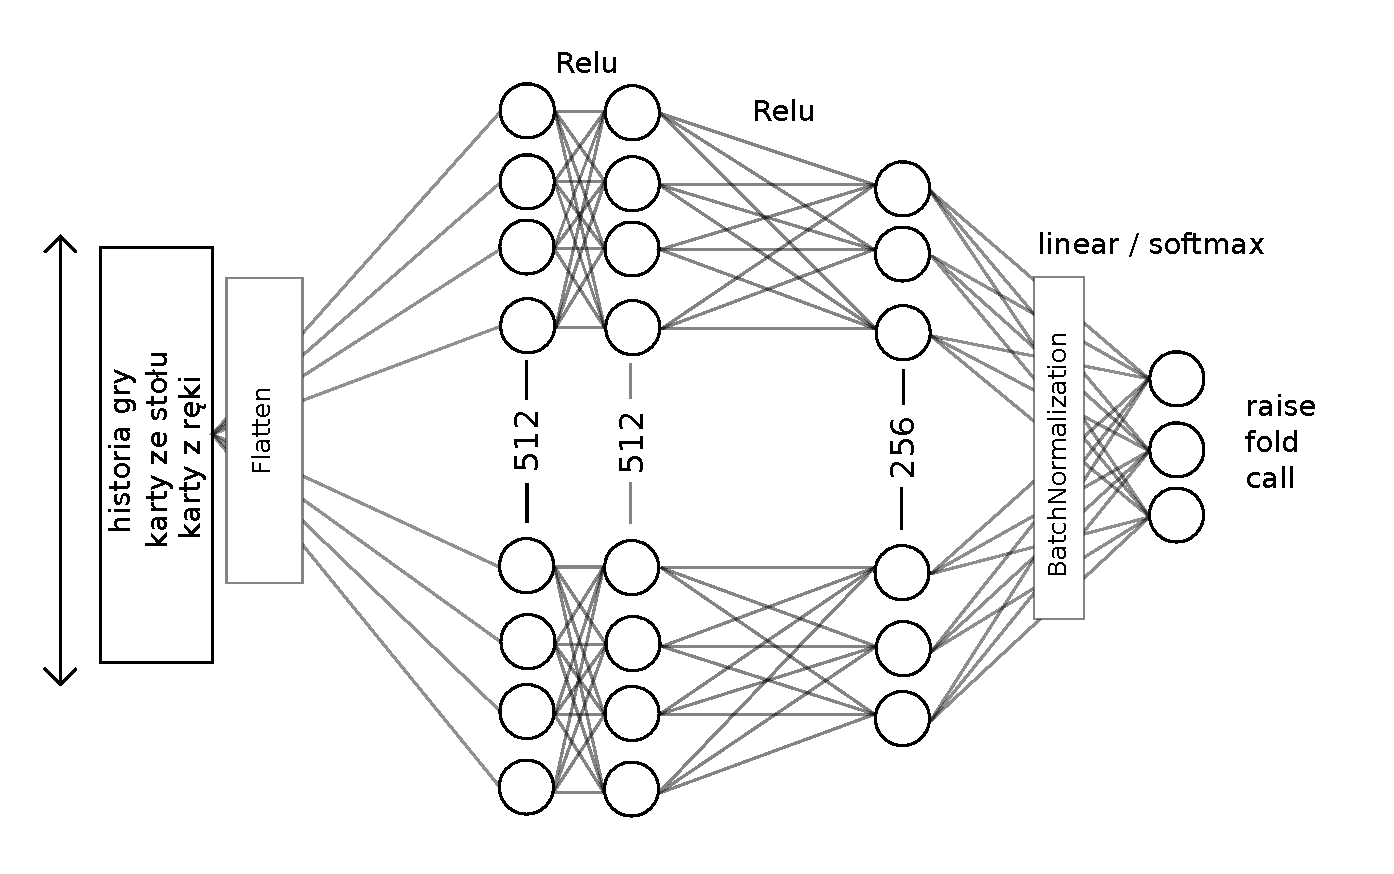
\includegraphics[width=1\textwidth]{./img/nn.pdf}
  \caption{Architektura sieci neuronowych wykorzystana w programie.}
\end{figure}

\subsection{Budowa zbiorów danych}

Jak wynika z algorytmu Deep CFR, w programie muszą być zawarte trzy bufory.
Maksymalna pojemność kontenerów $B_{1}$ i $B_{2}$ jest równa 300 000 próbek.
Bufor $B_{s}$ może posiadać ich 600 000. Każdy z dodawanych elementów do bufora składa się z
trzech połączonych wektorów o rozmiarach 52. W tym celu
zaimplementowano klasę $\emph{Memory}$ zarządzającą tymi zbiorami. Działają one jak 
kolejki i posiadają typ danych \emph{deque} co oznacza, że
w przypadku przepełnienia jest usuwany najstarszy wpis.

Mając uzupełnione dane w tablicach, program rozpoczyna przygotowanie zbiorów danych do uczenia
wybranych
sieci neuronowych. Każdy z buforów zostaje losowo przetasowany i podzielony na dwa podzbiory.
Pierwszy z nich to zbiór uczący zajmujący 80\% całej bazy. Wykorzystuje się go do poprawiania wag modelu sekwencyjnie.
Drugim zbiorem
są dane walidacyjne. Dokonanie takiego podziału było wymagane, aby przeciwdziałać stanowi
przetrenowania modelu. Zbiór walidacyjny jest nadzorowany i na jego podstawie można określić 
moment od którego model przestaje dobrze działać. Schemat tego
podziału przedstawiono na rys. 3.2. 
Dodatkowo w trakcie nauki sieć neuronowa aktualizuje swoje wagi w każdym kroku przez użycie elementu o nazwie
\emph{minibatch}, będącym parametrem określającym
mały podzbiór bazy użyty do trenowania sieci w pojedynczym kroku. Jego liczebność jest równa 500
próbek.

\begin{figure}[!ht]
  \centering
  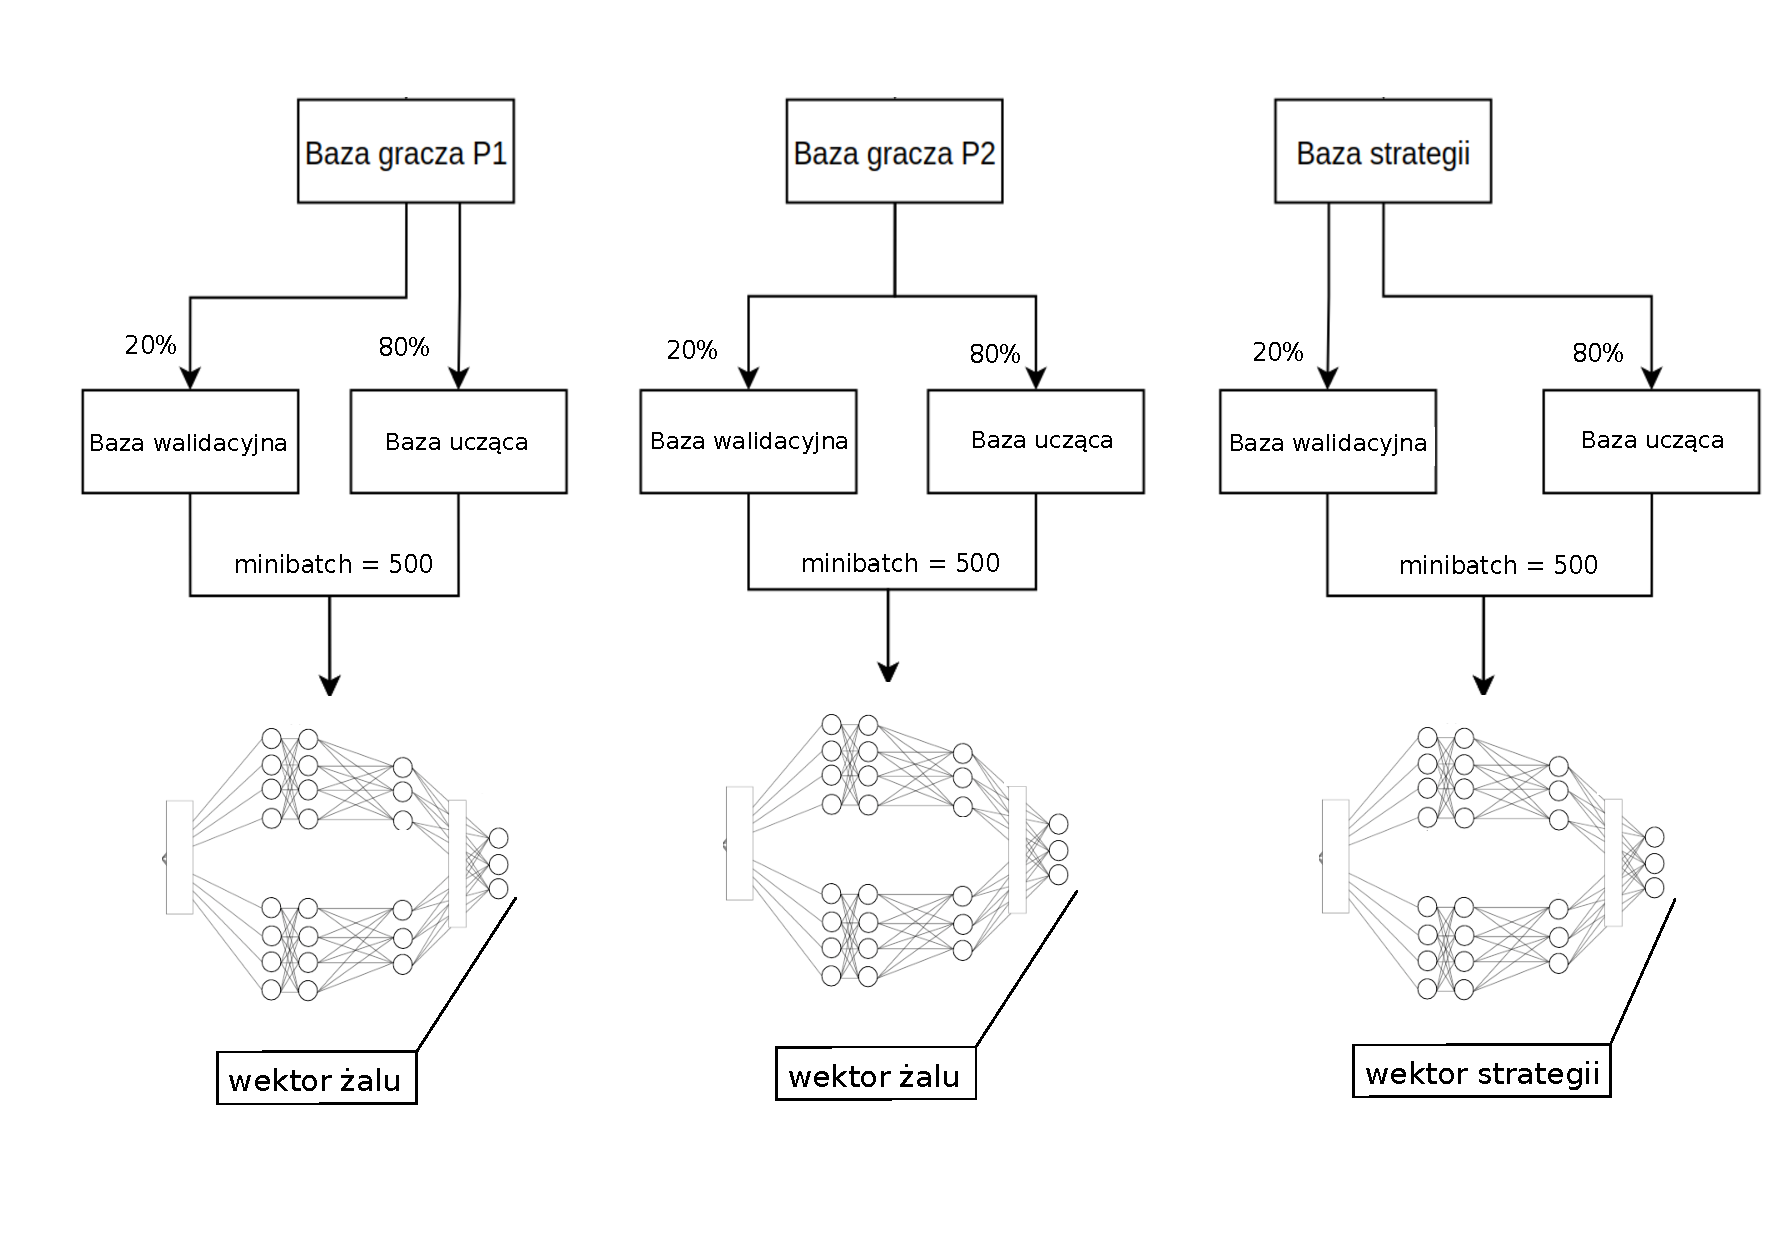
\includegraphics[width=1\textwidth]{./img/bzd.pdf}
  \caption{Podział danych.}
\end{figure}


\subsection{Proces uczenia}

Algorytm Deep CFR do gromadzenia obserwacji w buforach wykorzystuje metodę MCCFR ES, która eksploruje w jednej iteracji
wiele razy drzewo decyzyjne.
Po zakończeniu 
wszystkich powtórzeń zachodzi etap uczenia jednej z sieci neuronowych $\theta_{1}$, $\theta_{2}$
wykonując maksymalnie 5 000 aktualizacji wag pod warunkiem jeśli wcześniej nie dojdzie do dużych
oscylacji błędu predykcji w zbiorze walidacyjnym.
Taki schemat działania jest wykonywany dla obu graczy i powtarza się wielokrotnie. Końcowym
zadaniem jest wytrenowanie sieci neuronowej $\theta_{s}$.  
Wszystkie te elementy zostały połączone przez klasę $\emph{Brain}$, agregującą obiekty
$\emph{Memory}$
oraz $\emph{Poker\_network}$, rys. 3.4. 

W celu śledzenia i zatrzymania oscylacji wyników uczenia, które mogły by doprowadzić model
do przetrenowania,
użyto funkcji \emp{EarlyStopping} \cite{tensorflow}.
Zatrzymuje ona iteracje modelu w przypadku kiedy błąd predykcji na zbiorze
walidacyjnym wzrośnie odpowiednio wysoko. Sprawdza się to na podstawie argumentu \emph{patience},
który określa próg, po którym nauka się kończy. Taka procedura została zastosowana, aby
polepszyć umiejętność generalizacji wyników przez model, a wraz z tym zwiększyć jego jakość \cite{early}.
Rys. 3.3 prezentuje przykładowy punkt zakończenia nauki modelu w momencie przekroczenia progu
\emph{patience}.

Do samego trenowania sieci neuronowych wybrano urządzenie GPU GeForce GTX 1050. Wynika to z
uzyskiwania szybszych
rezultatów w przeciwieństwie do innej możliwości, jaka jest wykorzystanie CPU.

\begin{figure}[!ht]
  \centering
  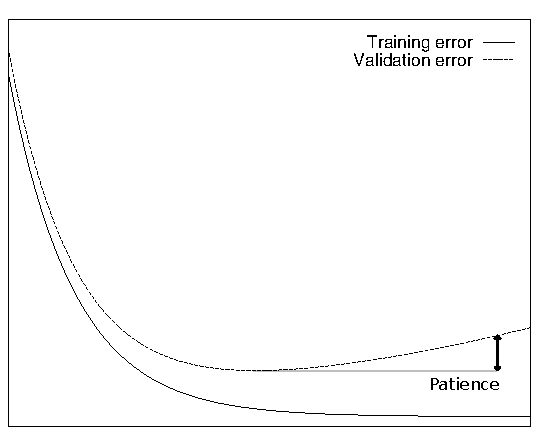
\includegraphics[width=0.6\textwidth]{./img/early.pdf}
  \caption{Przykład działania funkcji \emph{EarlyStopping} \cite{early}.}
\end{figure}

\vspace{2cm}


\section{Implementacja środowiska}

Do symulacji gry HULH z którą model będzie się komunikował, użyto biblioteki PyPokerEngine \cite{PPE}.
Klasa 
\emph{HULH\_Emulator} 
zaimplementowana w programie pozwala na utworzenie obiektu
zarządzającego taką grą. Przy tworzeniu go zostają zdefiniowane 
nazwy graczy \emph{P1} i \emph{P2}, które pełnia rolę identyfikatorów.
W dalszej części działania algorytmu są używane do śledzenia historii gry oraz wykonywania
wszelkich akcji graczy. 
W tabeli nr 3.3 wylistowano parametry ustawione w programie, do rozpoczęcia nauki.


\begin{table}[h!]
\centering
\caption{Parametry gry HULH.}
\begin{tabular}{|c|c| }
   \hline
   parametr & wartość \\
    \hline
   ante & 0  \\ 
   \hline
   mała w ciemno & 5  \\  
   \hline
   duża w ciemno & 10 \\
   \hline
   liczba rund po których resetuje się środowisko & 1  \\
   \hline
   udział każdego z graczy (stock) & 80  \\
   \hline
   liczba graczy & 2 \\
   \hline
\end{tabular}
\end{table}

\vspace{0.5cm}

Zaimplementowane środowisko po każdej wprowadzonej akcji zwraca dwa
elementy, obiekt \emph{State} określający stan gry oraz historię gry w formie słownika. 
Obie wartości są używane do
śledzenia postępu gry oraz pozycji w drzewie decyzyjnym. Dzięki takim obiektom \emph{HULH\_Emulator}
może
zwrócić graczowi informacje o dostępnych kartach, historii gry lub 
wygranych stawkach z dowolnego stanu wprowadzonego przez model.  

Zaimplementowana gra symuluje HULH, czyli działa w taki sposób, że 
każde podbicie stawki jest wielkości
dużej w ciemno. Dzięki takiemu założeniu gra nie kończy się zbyt szybko 
pod warunkiem, że żaden z graczy nie wykona akcji \emph{fold}. Dodatkowo ustalono, że po
każdej 
rundzie środowisko jest resetowane. Taki proces został ustawiony na czas uczenia.
Powodem jest powstawanie mniejszych drzew
decyzyjnych, co pozwala na szybszą naukę modeli oraz krótszy czas poświęcany na eksplorację
gry przez
MCCFR ES. W etapie rozgrywek między modelami gra będzie kończyć się dopiero po wyczerpaniu 
się żetonów po jednej ze stron.


\section{Implementacja Deep CFR}

Klasa \emph{DCFR} zawiera implementację algorytmu Deep CFR. 
Przy tworzeniu obiektu powstają razem z nim
trzy elementy klasy \emph{Brain}, gracz, oponent oraz strategia $\sigma$ .
Do tego ustawiane jest środowisko \emph{HULH\_Emulator} przez referencje.

Cały proces powstawania modelu rozpoczyna się od funkcji \emph{iterate}, która wykonuje trzy pętle
\emph{for},
dla iteracji algorytmu po 50 razy oraz powtórzeń eksploracji drzewa dla każdego z gracza po 270 razy. W pierwszej z nich 
środowisko tworzy nową grę, w ostatniej pętli jest wykonywana funkcja \emph{\_\_traverse},
działająca według metody MCCFR ES. Dostaje ona argumenty \emph{state} czyli obiekt określający
stan gry, \emph{events} - dotychczasową historię oraz \emph{timestep}.
Ostatni argument \emph{verbose} jest opcjonalny i służy tylko do wizualizacji powstałego drzewa
decyzyjnego. Wszystko działa przez rekurencję w celu stworzenia drzewa decyzyjnego.
Po zakończeniu działania MCCFR ES rozpoczyna się uczenie sieci neuronowej $\theta_{p}$.
Po wszystkich powtórzeniach rozpoczyna się trenowanie sieci $\theta_{s}$ oraz zapisanie jej w formie
pliku. Aby spełnić warunek 
utworzenia pięciu modeli, kolejno ustawiono w funkcji \emph{iterate} opcjonalny argument
\emph{checkpoint}. Przyjmuje on bazową wartość \emph{None}. Przy uruchamianiu programu zmieniono 
ją na liczbę 10, co oznacza, że co 10 iteracji będzie trenowana sieć $\theta_{s}$ z uzbieranego bufora
i zapisywana. 

Po ustawieniu wszystkich parametrów uruchomiono program, który wykonywał się przez trzy dni.
Tab. 3.4 prezentuje podstawowe parametry zaimplementowanego algorytmu.

\vspace{1cm}
\begin{table}[h!]
\centering
\caption{Parametry algorytmu Deep CFR.}
\begin{tabular}{|c|c| }
   \hline
   parametr & wartość \\
    \hline
   liczba powtórzeń eksploracj drzewa & 270  \\ 
   \hline
   liczba iteracji algorytmu & 50  \\  
   \hline
   co ile iteracji wytrenować i zapisać model & 10 \\
   \hline
\end{tabular}
\end{table}

\newpage

\section{Podsumowanie}


W tym rozdziale zaprezentowano implementację algorytmu wraz z użytymi technologiami. Program
następnie został uruchomiony  z zadanymi parametrami jak 50 iteracji po 270 eksploracji drzewa.
Wykonywał się on przez okres czterech dni, używając GPU. Postępy
tworzonych pięciu modeli były na bieżąco analizowane i zapisywane. Przedstawiono 
między innymi strukturę sieci
neuronowych, budowę zbioru danych, działanie środowiska HULH oraz funkcje związane z uczeniem
algorytmu. Pokazano cel użycia takich metod jak \emph{EarlyStopping} lub \emph{Flatten}. Na rys. 3.4
przedstawiono dokładny schemat zaimplementowanego algorytmu.
Następny
rozdział przedstawi zapisane wyniki ilustrujące jakość utworzonych modeli oraz sprawdzi, który z
nich będzie najlepiej grał w HULH.

\vspace{1cm}

\begin{figure}[!ht]
  \centering
  \hspace*{-1cm}   
  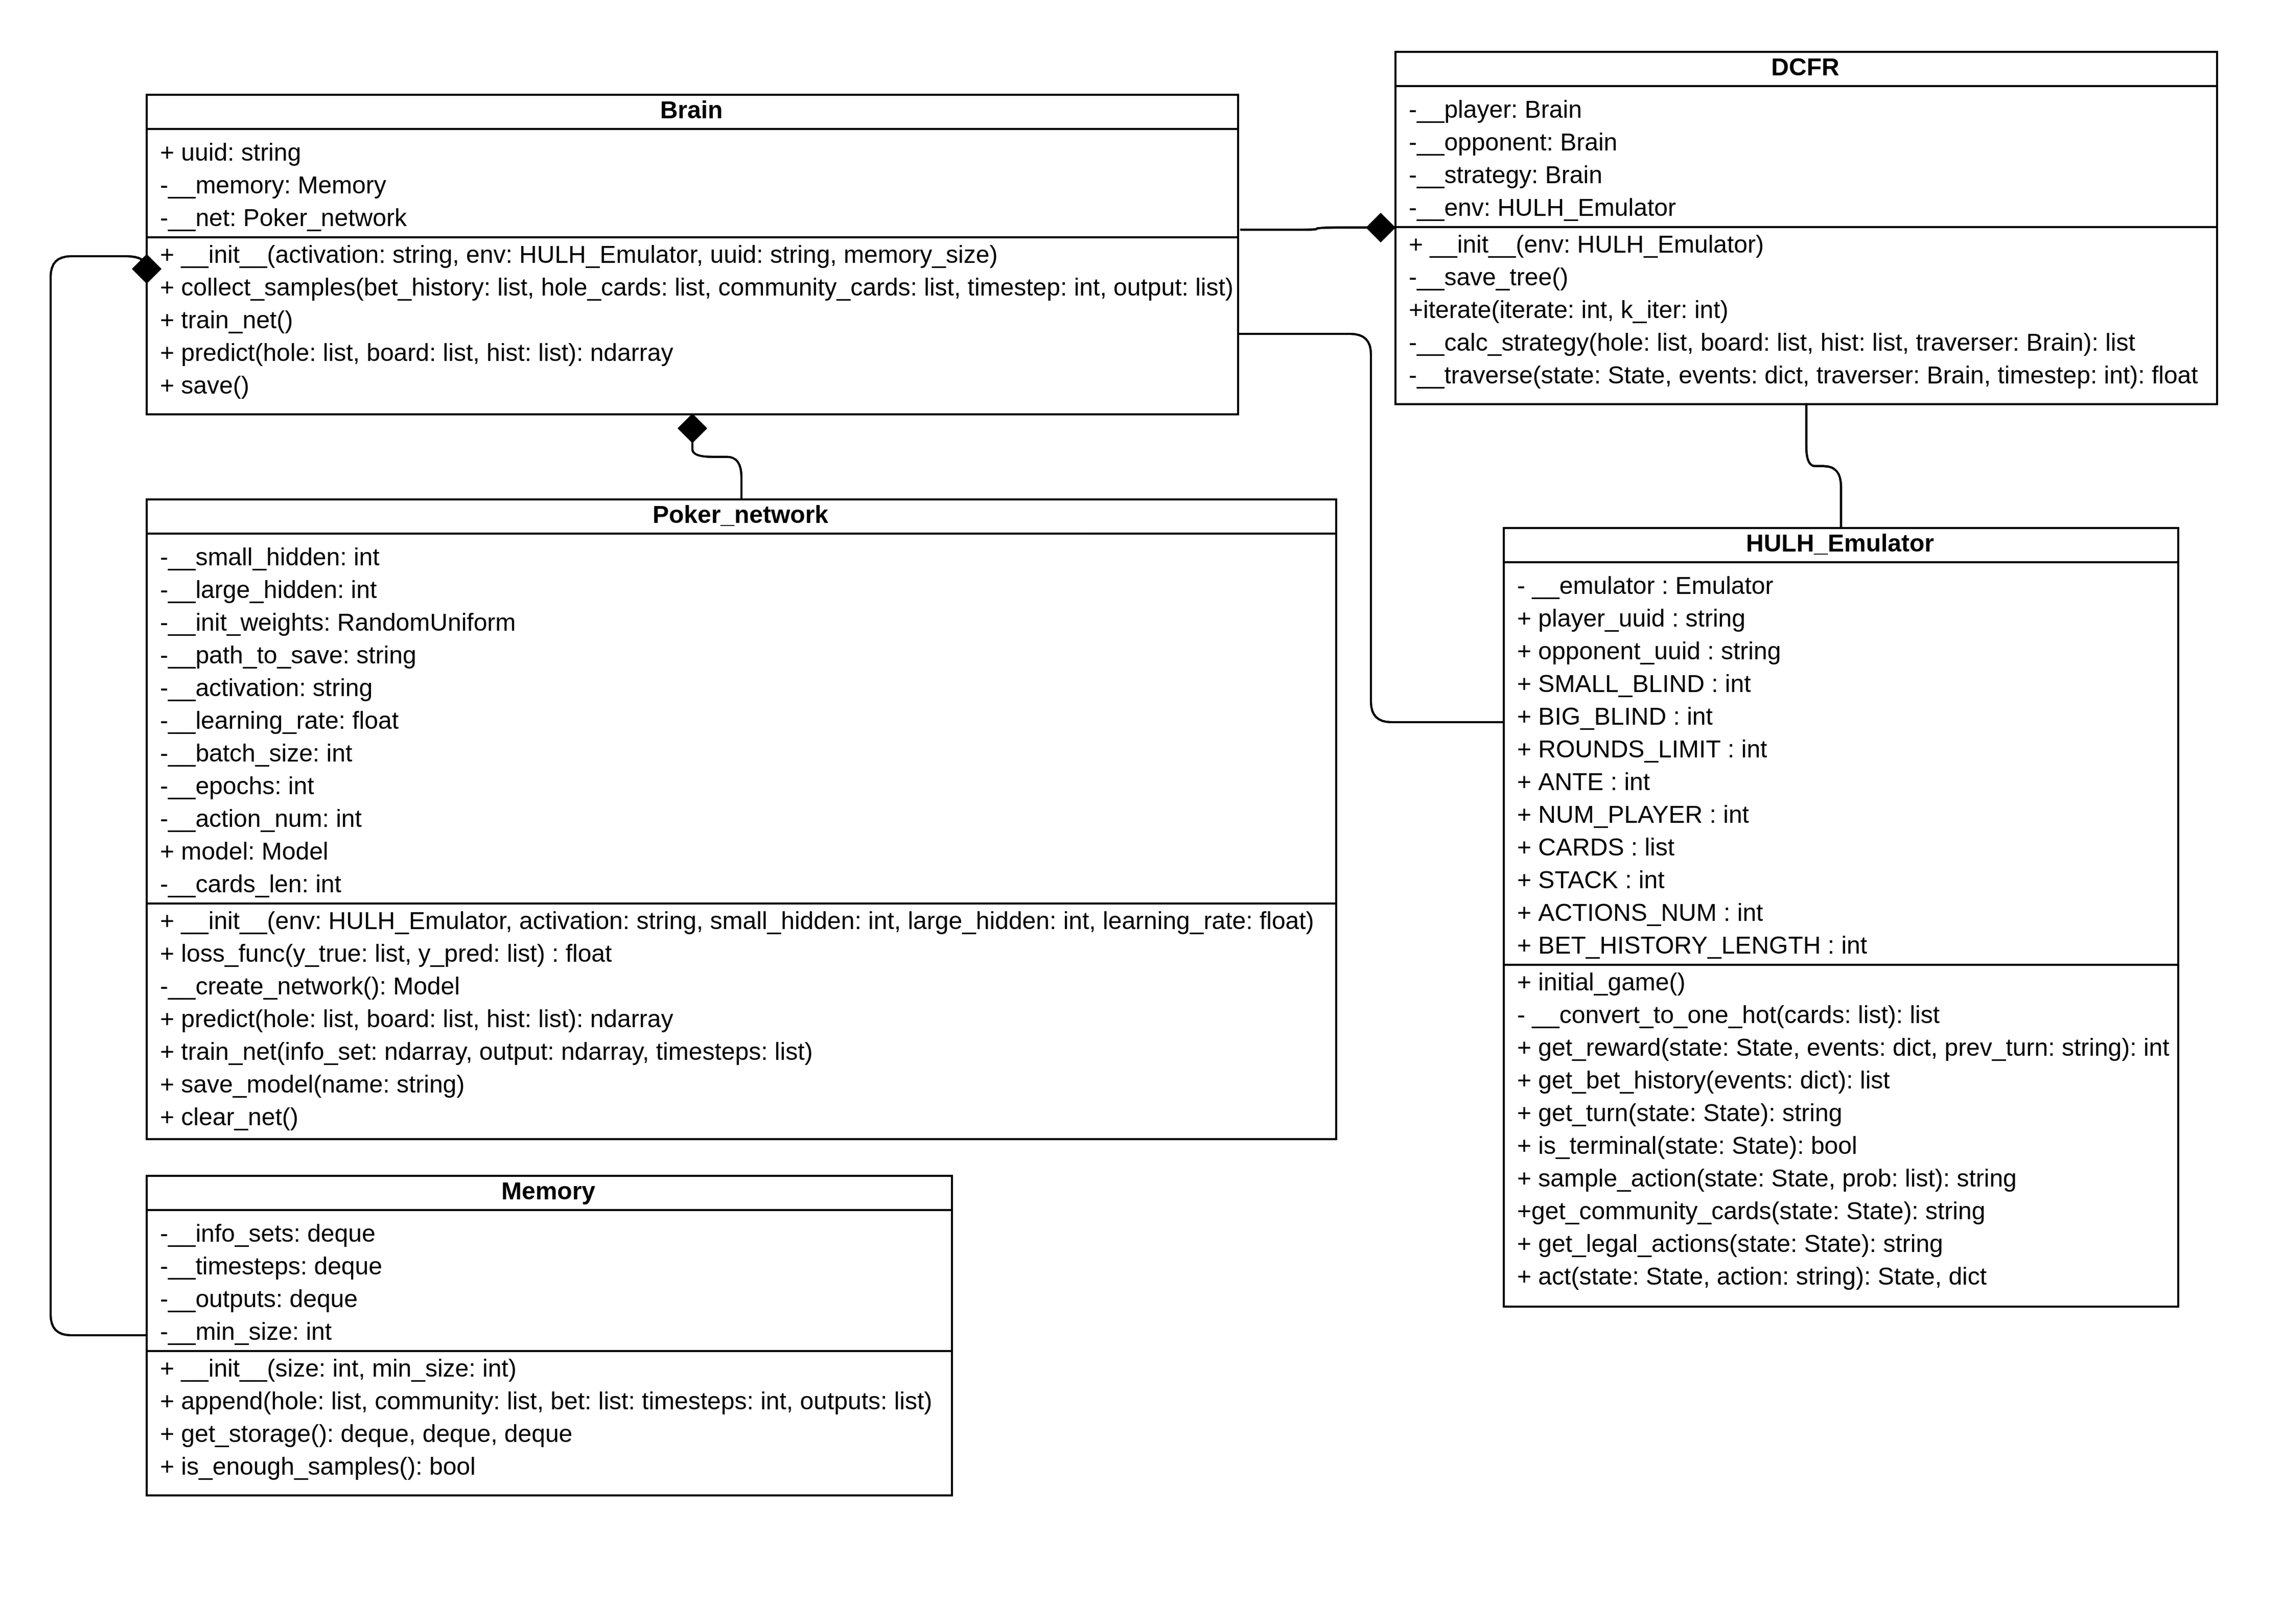
\includegraphics[width=1.1\textwidth]{./img/uml.pdf}
  \caption{Diagram UML projektu.}
\end{figure}





\chapter{Wyniki}

Rozdział przedstawia rezultaty powstałe po około czterech dniach nauki modelu. Celem rozdziału jest 
przedstawienie wyników uczenia oraz rezultatów
wszystkich rozgrywek między modelami.
Dodatkowo, aby przedstawić jakość algorytmu, najlepsze modele zagrają 200 razy z prostym
programem zawartym w bibliotece PyPokerEngine, który symuluje
gracza nigdy nieblefującego i niewykonującego akcji \emph{raise}.
Zostaną tutaj zaprezentowane różnice między utworzonymi AI wraz z ich przewidywaną jakością
korzystając z odpowiednich wykresów bazujących na danych pobranych z modułu \empg{TensorBoard}. 
Dodatkowo zostanie dokonana próba wyboru najlepszego modelu na podstawie
wszystkich etapów oraz klasyfikacji jego stylu gry.

\section{Proces uczenia modelów rozpoznawania}

Algorytm Deep CFR zdołał utworzyć pięć modeli rozpoznawania, gdzie każdy proces nauki
był
śledzony przez funkcje biblioteki \emph{TensorBoard}. Uzyskane dane następnie zostały
użyte do utworzenia czytelnych wykresów ilustrujących zależność błędu predykcji od liczby
iteracji.

Pierwsze utworzone AI powstał po 10 iteracjach metody Deep CFR, co zajęło około 5 godzin.
Następnie rozpoczęła się nauka sieci $\theta_{s}$ ze zbiorem danych $B_{s}$ zapełnionym przez około 300 000 próbek.
Można zauważyć na rys. 4.1,
że wartość błędu po 40 krokach uczenia nie zmieniła się mocno dla obu zbiorów.
W przypadku danych walidacyjnych sieć neuronowa przy dokonywaniu predykcji powodowała duże oscylacje
wartości, pozostając na poziomie około 2,2, co przyczyniło sie do zakończenia procesu przedwcześnie przez \emph{EarlyStopping}.
Przy takim okresie model zmniejszył błąd predykcji zbioru uczącego wynoszący początkowo 0,2 do wartości bliskiej 0.

Analizując taki wykres, można stwierdzić, że model nauczył się z zebranych danych zależności między
wprowadzanymi obserwacjami a zwracanymi akcjami. Dodatkowo rys. 4.6 pokazuje, że takie AI gra lepiej
względem wielu utworzonych później modeli.


\begin{figure}[!ht]
  \centering
  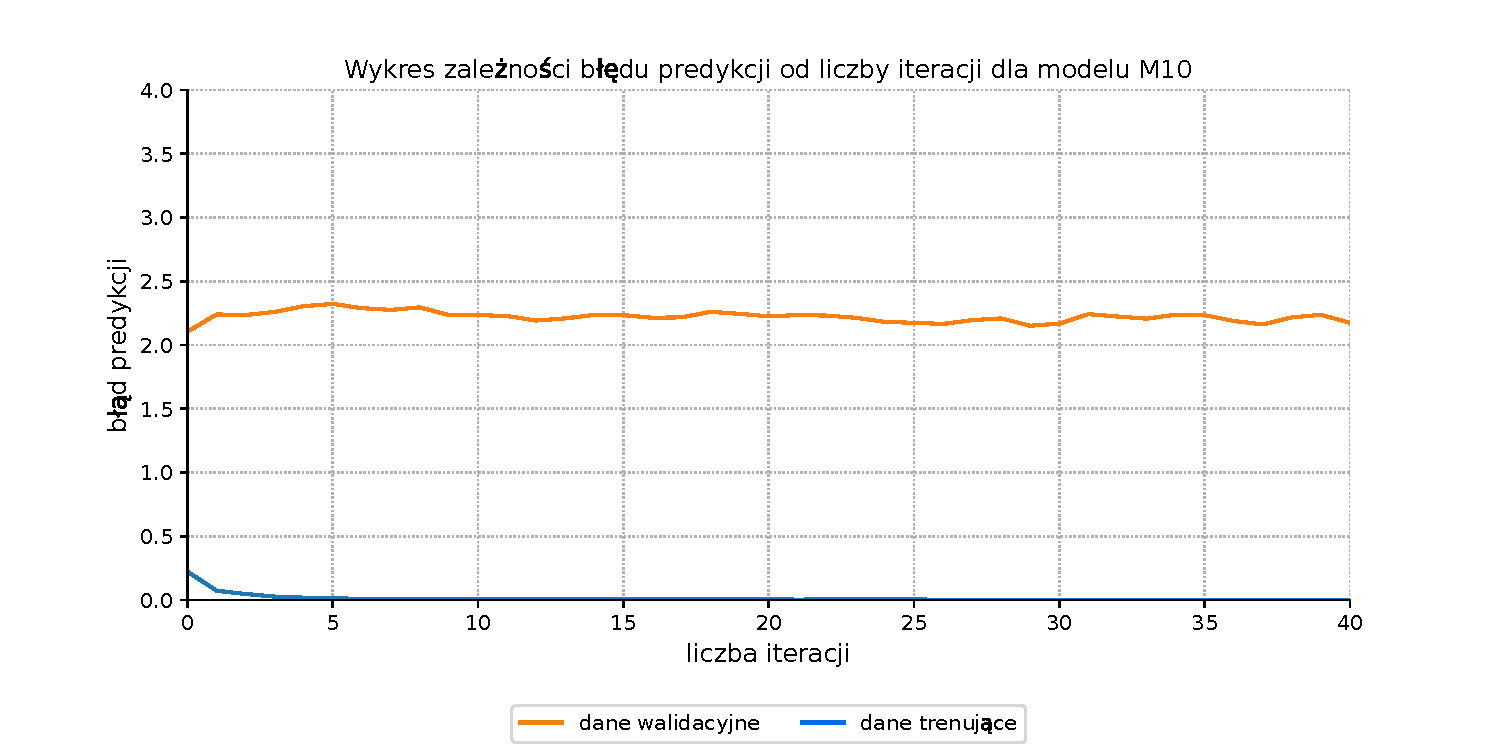
\includegraphics[width=0.9\textwidth]{./img/model1.pdf}
\caption{Wyniki uczenia modelu po 10 iteracjach Deep CFR.}
\end{figure}


\begin{figure}[!ht]
  \centering
  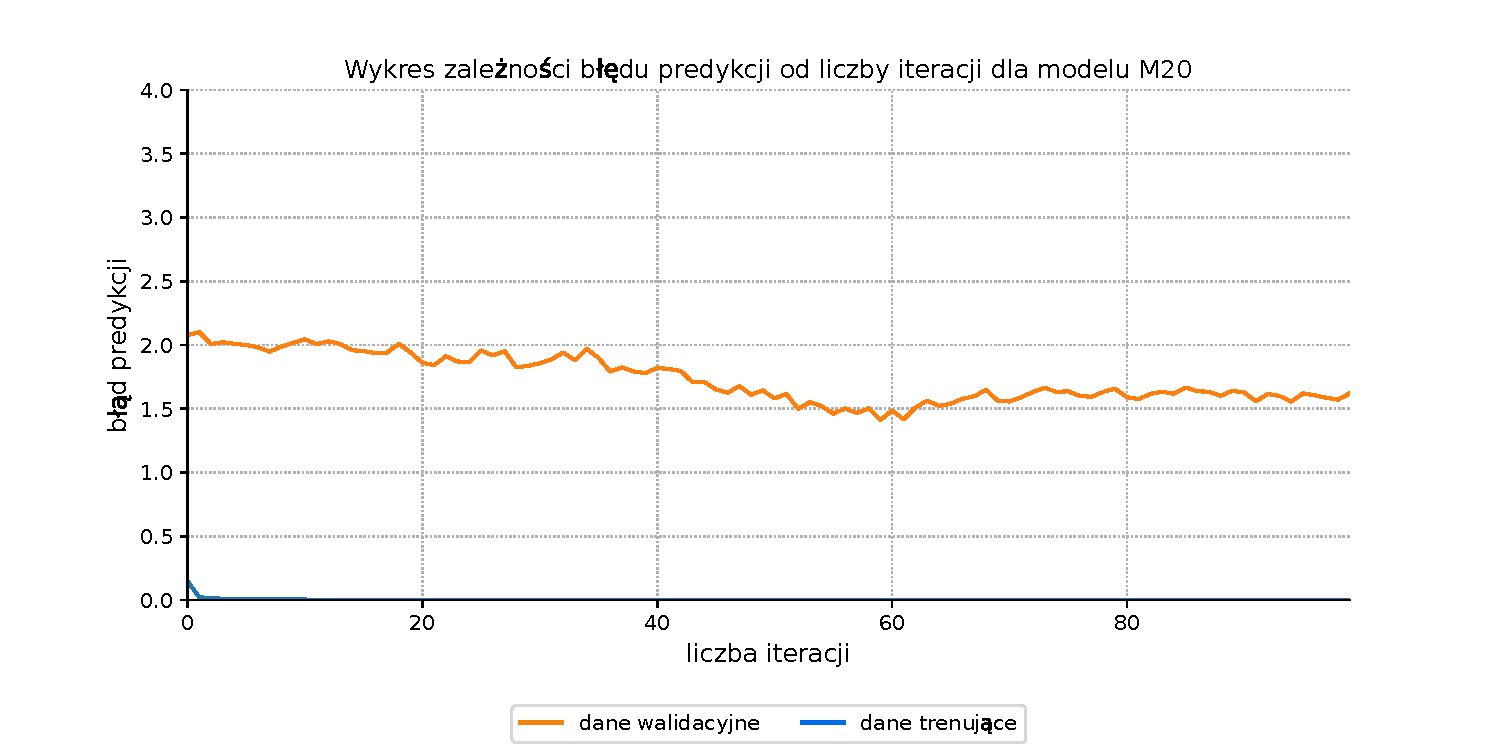
\includegraphics[width=0.9\textwidth]{./img/model2.pdf}
\caption{Wyniki uczenia modelu po 20 iteracjach Deep CFR.}
\end{figure}


\newpage
Po 20 powtórzeniach algorytmu Deep CFR utworzono drugi model rozpoznawania. 
Nastapiło to po około 12 godzinach. Algorytm do nauki użył prawie całego zapełnionego buforu $B_{s}$.
W zbiorze znajdowały się nowe próbki oraz te, które zebrano przed nauką pierwszego AI.
Proces uczenia przebiegał początkowo w podobny sposób jak w poprzednim etapie. Model zaczął od błędu
predykcji 2,2 dla zbioru walidującego i błędu 0,2 dla buforu uczącego. Pierwszą różnicą względem 
poprzedniego etapu jest lepsza nauka na podstawie buforu walidacyjnego, po 10
powtórzeniach wartości zaczęły mocno
maleć aż do błędu predykcji wynoszącej około 1,4. Następnie pojawił się krótki wzrost wartości i
utrzymywanie się
na tym samym poziomie z lekkimi oscylacjami co spowodowało 
zakończenie procesu. Wykres 4.2 dobrze pokazuje cel używania biblioteki \emph{EarlyStopping}.
Prawdopodobnie przy większej liczbie iteracji model zacząłby uzyskiwać coraz gorsze wartości
predykcji zbioru walidacyjnego. Podsumowując, model uzyskał lepsze wyniki względem etapu pierwszego,
co może wynikać z większego zbioru danych. Rys. 4.6 pokazuje, że utworzony
model wygrywa nieznacznie z AI M10 przy 200 powtórzonych grach.

Kolejne AI zostało wytrenowane po 30 iteracjach. Był to drugi dzień działania algorytmu
Deep
CFR. W tym momencie bufor $B_{s}$ był całkowicie zapełniony, przez co
nowe próbki dodawane do zbioru usuwały najstarsze wpisy. Na tak dużej bazie model uczył się 
przez około 100
powtórzeń. Nauka modelu na podstawie zbioru uczącego była podobna jak w poprzednich etapach. Główną
różnicą jest bufor walidacyjny, dla którego błąd początkowo wyniósł 3,5 i zmalał do 1,7. 

\vspace{0.5cm}

\begin{figure}[!ht]
  \centering
  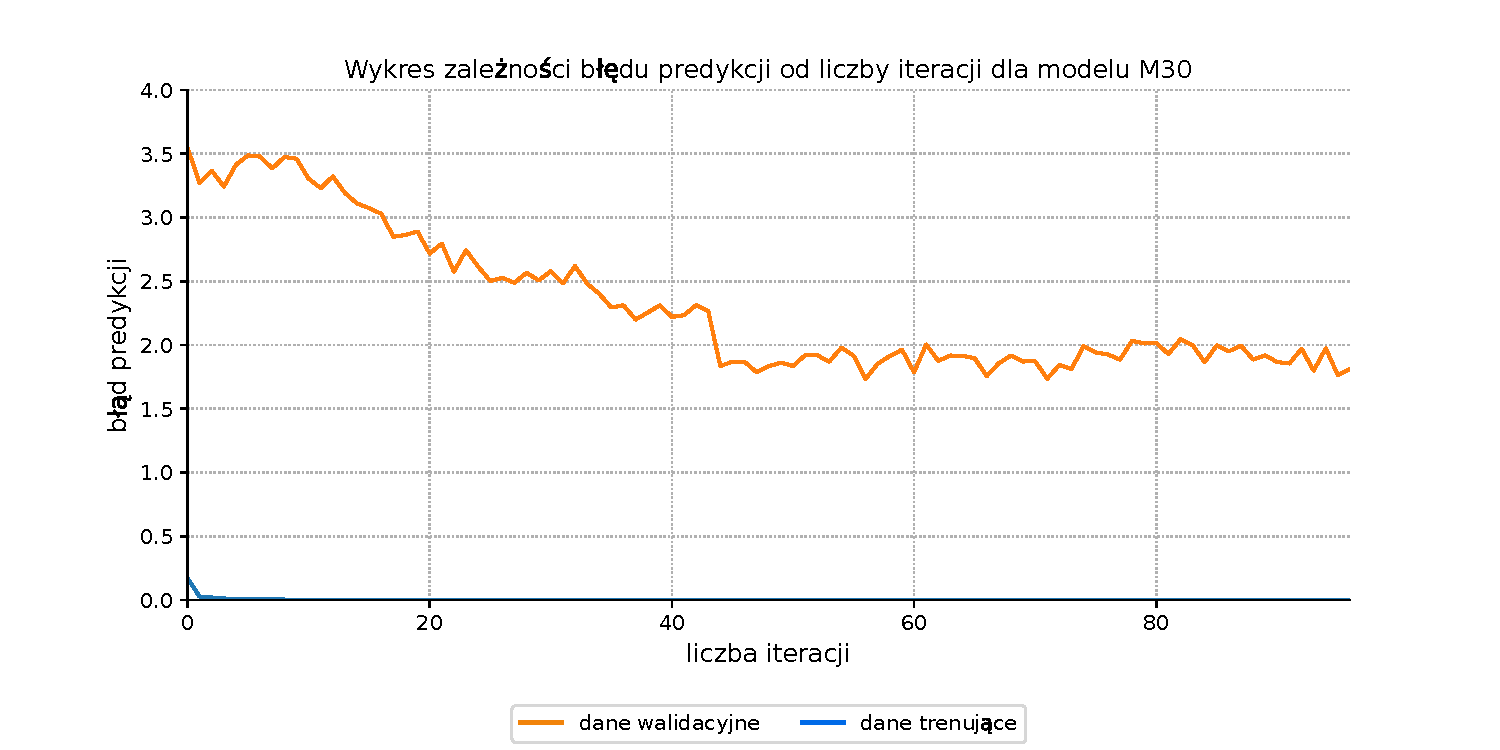
\includegraphics[width=0.9\textwidth]{./img/model3.pdf}
\caption{Wyniki uczenia modelu po 30 iteracjach Deep CFR.}
\end{figure}


\begin{figure}[!ht]
  \centering
  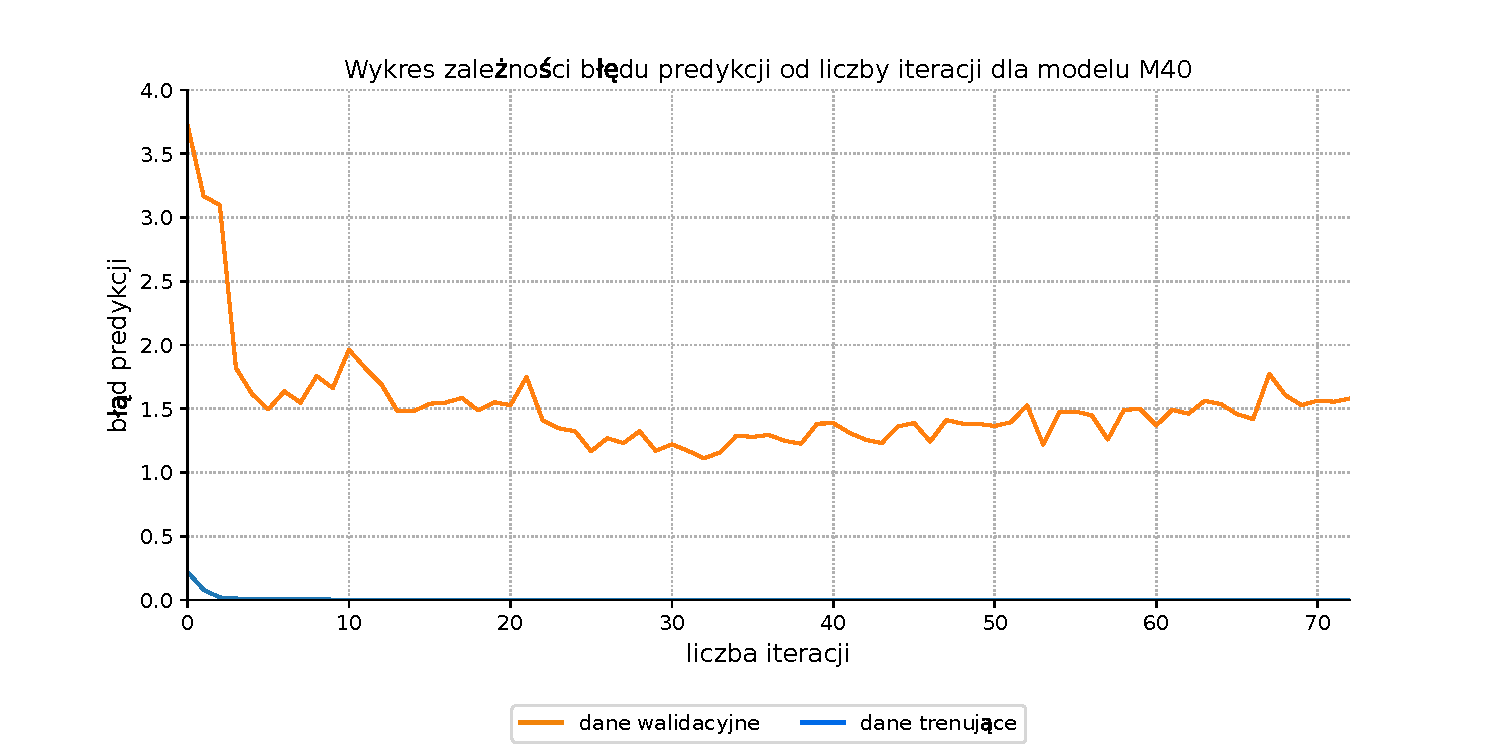
\includegraphics[width=0.9\textwidth]{./img/model4.pdf}
\caption{Wyniki uczenia modelu po 40 iteracjach Deep CFR.}
\end{figure}

Model nr 4 powstał po 40 iteracjach. Wytrenował sieć neuronową po około 75 potwórzeniach gdzie 
wartości błedu predykcji prezentuja sie w podobny sposób jak w poprzednim etapie. Jedyną róznicą
jest gwałtowny spadek błędu predykcji w pierwszych 5 iteracjach.

Ostanie AI utworzono po 4 dniach. Rys. 4.5 pokazuje, że proces nauki przebiegał początkowo z 
niewielkim błędem predykcji i powoli sie zmniejszał do wartości 1,9 w przypadku zbioru walidacyjnego.
Drugi zbiór doprowadził do podobnych rezoltatów jak we wszystkich etapach.

\begin{figure}[!ht]
  \centering
  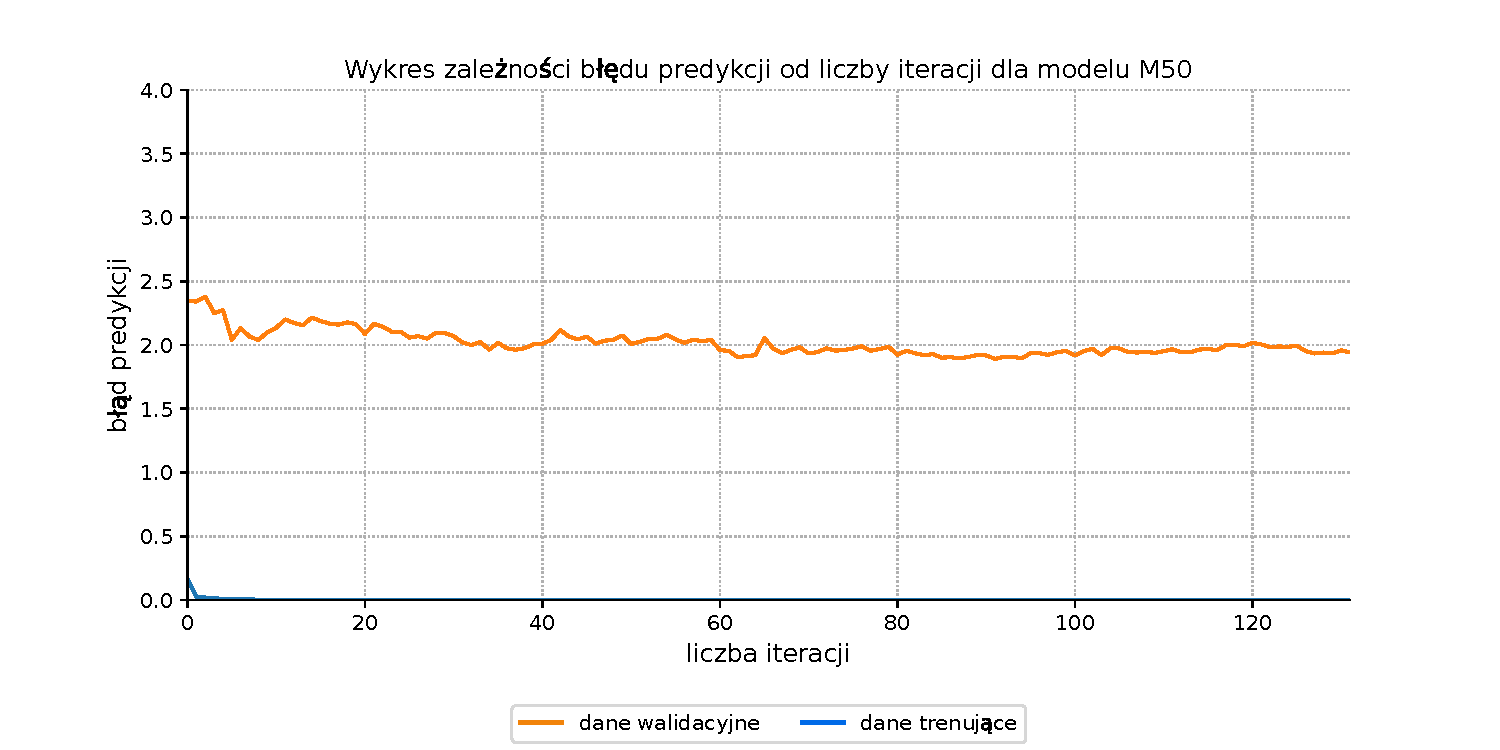
\includegraphics[width=0.9\textwidth]{./img/model5.pdf}
\caption{Wyniki uczenia modelu po 50 iteracjach Deep CFR.}
\end{figure}

Podsumowując powyżesze wyniki można stwierdzić, że zbierane dane w buforze $B_{s}$
przez Deep CFR są łatwe w znajdowaniu zależności. Główną przyczyną mogą być dane 
wejściowe i wyjściowe o niewielkim rozmiarze wraz z prostym środowiskiem.
Prawdopodobnie przy grach dłuższych niż jedna runda, gdzie gracz przegrywa dopiero jak straci 
wszystkie żetony, oraz przy większym zbiorze informacji wejściowych proces uczenia by nie 
przebiegał tak szybko. W takim przypadku model by musiał uwzględnić dodatkowe czynniki jak 
numer rundy, liczba pozostałej sumy żetonów gracza lub przewaga przeciwnika. 


\vspace{1cm}
\begin{table}[th!]
\centering
\caption{Lista utworzonych modeli.}
\begin{tabular}{|c|c|c| }
   \hline
   nazwa modelu & liczba iteracji Deep CFR & liczba aktualizacji wag $\theta_{s}$ \\
    \hline
   M10 & 10 & 40 \\ 
   \hline
   M20 & 20 & 98  \\  
   \hline
   M30 & 30 & 92 \\
   \hline
   M40 & 40 & 73 \\
   \hline
   M50 & 50 & 131 \\
   \hline
\end{tabular}
\end{table}


\section{Wyniki rozgrywek modeli}


W celu przetestowania jakości utworzonych modeli przeprowadzono 10 
rozgrywek gdzie każda z nich to
pojedyncza kombinacja dwóch AI. Każdą grę powtórzono 200 razy z wieloma rundami tak, aby
zminimalizować czynnik losowości i zakończyć grę w momencie wyczerpania się żetonów po jednej ze
stron.
Następnie sporządzono cztery wykresy
ilustrujące wyniki tych rozgrywek. Rys. 4.6 przedstawia każdą kombinację gier 
z przypisaną liczbą 
wygranych każdemu z modeli. Rys. 4.7 i 4.8 mają za zadanie pokazać średnią wygrywanych i przegrywanych
pul przez graczy, a rys. 4.9 pokazuje rozkład wykonanych akcji. Takie wykresy pozwolą stwierdzić, który z modeli częściej wygrywa, ale też częściej
ryzykuje, przegrywając więcej, a który gra ostrożniej. 
 
\begin{figure}[!ht]
  \centering
  \hspace*{-1cm}   
  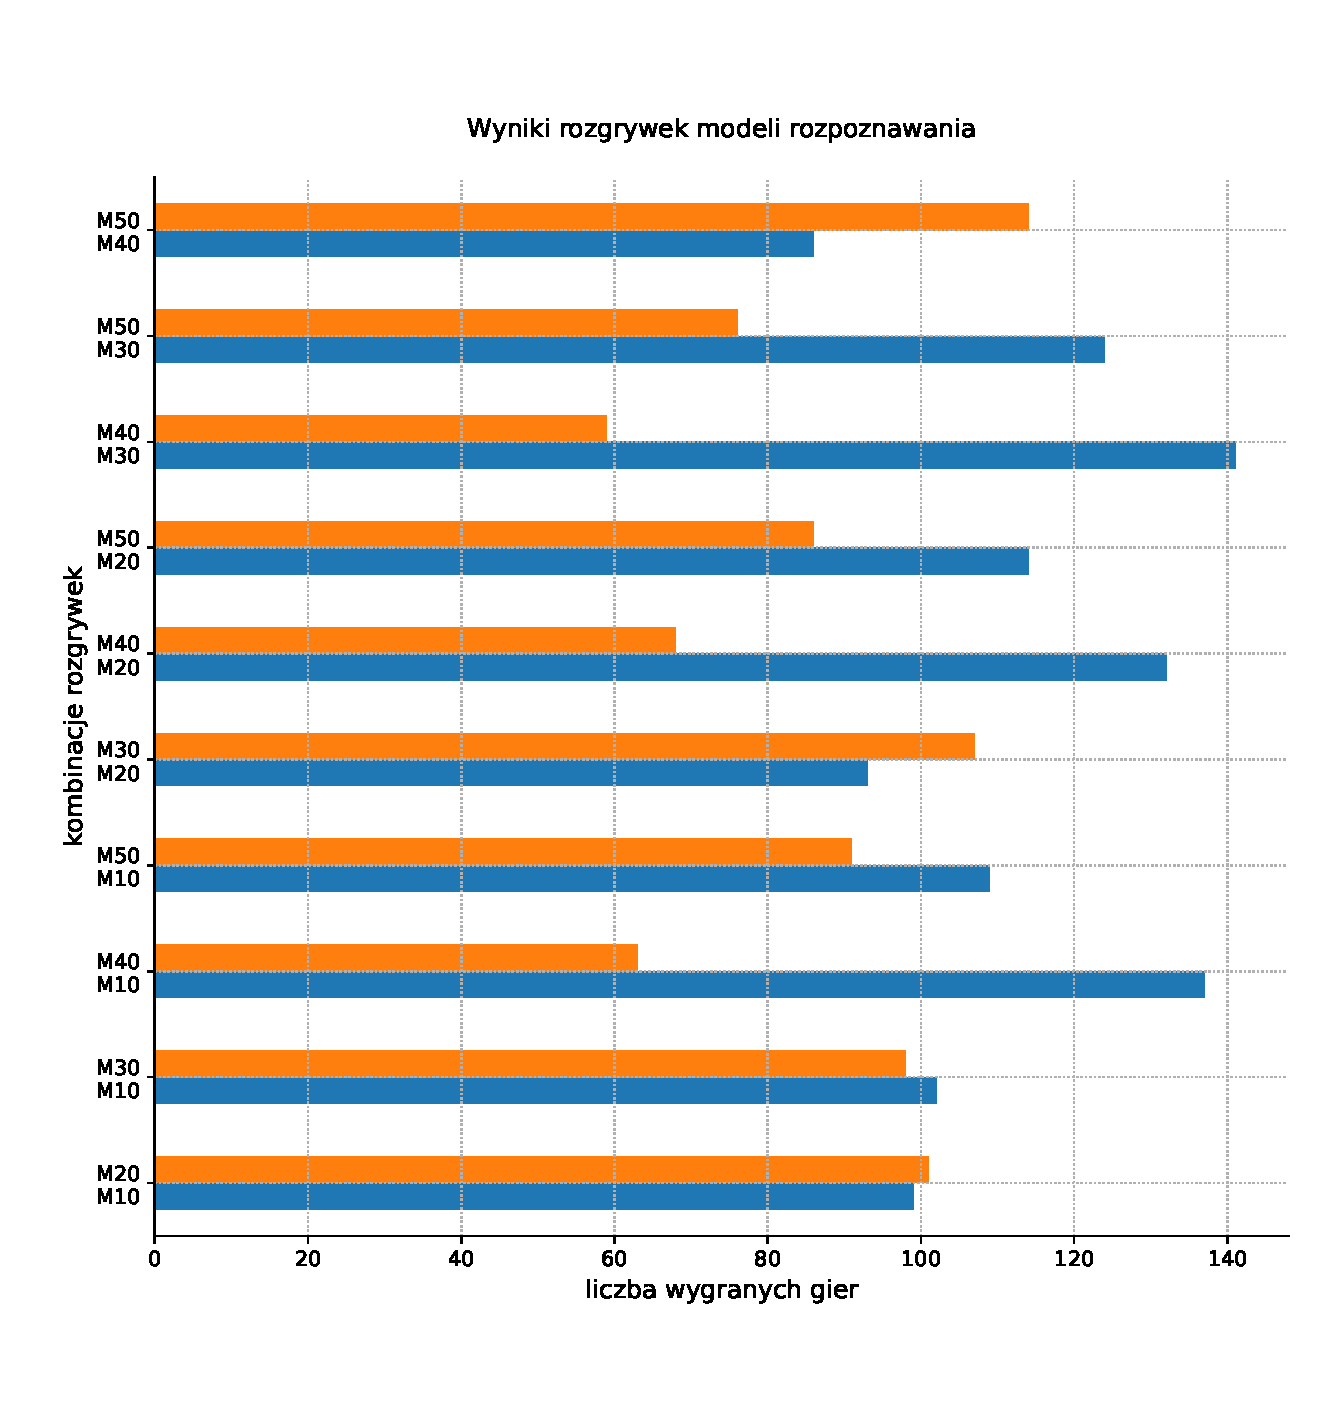
\includegraphics[width=0.9\textwidth]{./img/mecze.pdf}
  \caption{Kombinacje rozgrywek między utworzonymi modelami.}
\end{figure}


\vspace{3cm}
Analizując rys. 4.6 można zauważyć, że model 1 wygrywał z większością utworzonych AI najczęściej.
Największą przewagę  
zdobył względem modelu M40, około 140 wygranych względem 60 porażek oraz około 110 zwycięstw z
M50. Rozgrywki z resztą
uczestników, 
cechuje się niewielkimi przewagami gracza.
Wyjątkiem jest gracz M20, którego wybrane strategie okazały się skuteczne przeciwko oponentowi M10.
Przy wielokrotnym powtarzaniu eksperymentu, modele M30 i
M20 zdobywały lepsze lub gorsze wyniki niż M10 przez występujący w grze czynnik losowości. Podsumowując,
gracz pierwszy nieznacznie częściej wygrywał w porównaniu M30 i M20
przez co ciężko stwierdzić czy jest od nich lepszy.

Kolejny obiekt zdobywający najlepsze wyniki
to M30. Wygrał on z modelem M20 z dużą przewagą. Oznacza to, że wybierane strategie przez niego
są skuteczne w rozgrywce z takim typem przeciwnika. Dodatkowo osiągnął on tak samo 
dużą różnicę między wygranymi a przegranymi z modelem M40. 
Na podstawie takich informacji można stwierdzić, że AI powstałe po 40 iteracjach przegrywa
najczęściej,
a
utworzone w 1 i 3 etapie najrzadziej. W
dalszej części rozdziału zostanie zbadana możliwa przyczyna takich wyników.


Problemem wykresu rys. 4.6 jest pokazywanie tylko częstotliwości zwycięstw modeli, ale nie zawiera
informacji o sposobie gry każdego z graczy. 
Taka wiedza pozwoliłaby na stwierdzenie możliwych przyczyn powstałych
wyników.
W tym celu zebrano wszystkie wygrane wartości przez graczy z każdej rundy, a następnie
obliczono ich średnie. Rys. 4.7 przedstawia uśrednione wyniki przegrywanych puli przez każdego z
graczy, rys. 4.8 prezentuje odwrotną cechę. Analizując oba rysunki, można zauważyć, że model
nr 1, który posiada najwięcej wygranych, zyskuje i traci największą pulę w rundach.
Rys. 4.9 pokazuje też, że sztuczna inteligencja wykonuje równie często akcję \emph{call}
i \emph{raise}, ale bardzo rzadko akcję \emph{fold}. Jest
drugim najbardziej zrównoważonym graczem, który uzyskuje przy tym najbardziej skrajne wyniki.
Zaletą modelu jest to, że 
średnie wartości są na podobnym poziomie, co oznacza, że wygrywa i traci tyle samo. Bardzo podobnej
strategii używa gracz M50, ale pomimo tego przegrywa z omawianym modelem.
Gracz M30 okazał się graczem zyskującym i tracącym mniejsze wartości.
Może to wynikać z częstego wykonywania akcji \emph{call}. Modele M20, który znacznie
częściej wykonuje ten ruch, zdobywa najniższą pulę wygraną i przegraną.
Najgorsze wyniki ma gracz M40, który też najczęściej pasował. Uzyskał
on znacznie większą średnia wartość wygranej względem przegranej, ale najrzadziej wygrywał.


\newpage


\begin{figure}[!ht]
  \centering
  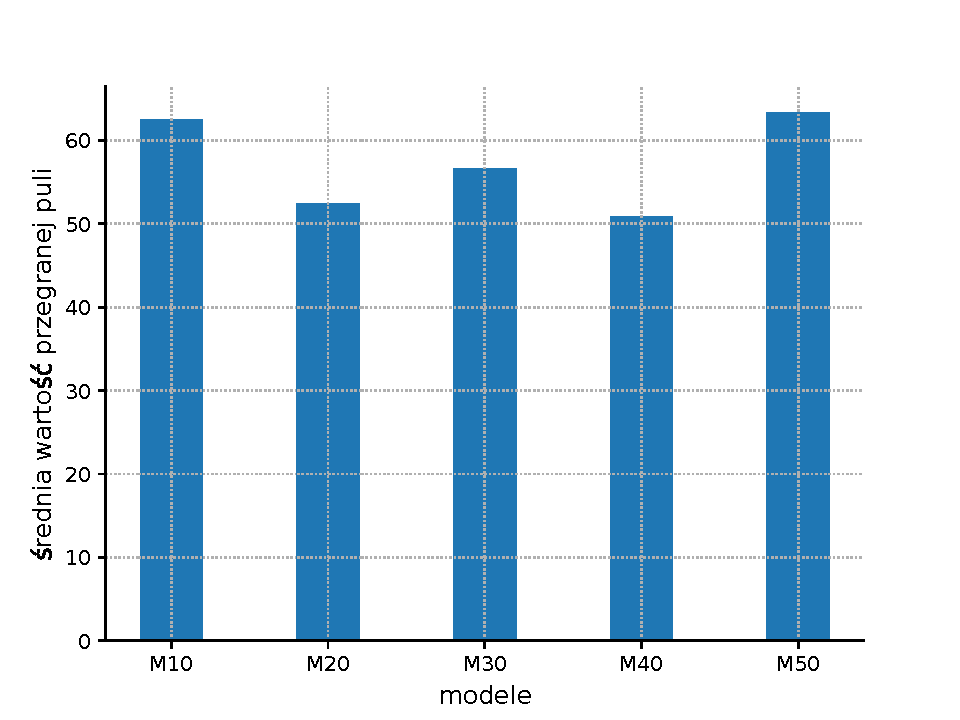
\includegraphics[width=0.75\textwidth]{./img/mecze_ps.pdf}
  \caption{Uśrednione wartości traconych żetonów przez modele.}
\end{figure}


\begin{figure}[!ht]
  \centering
  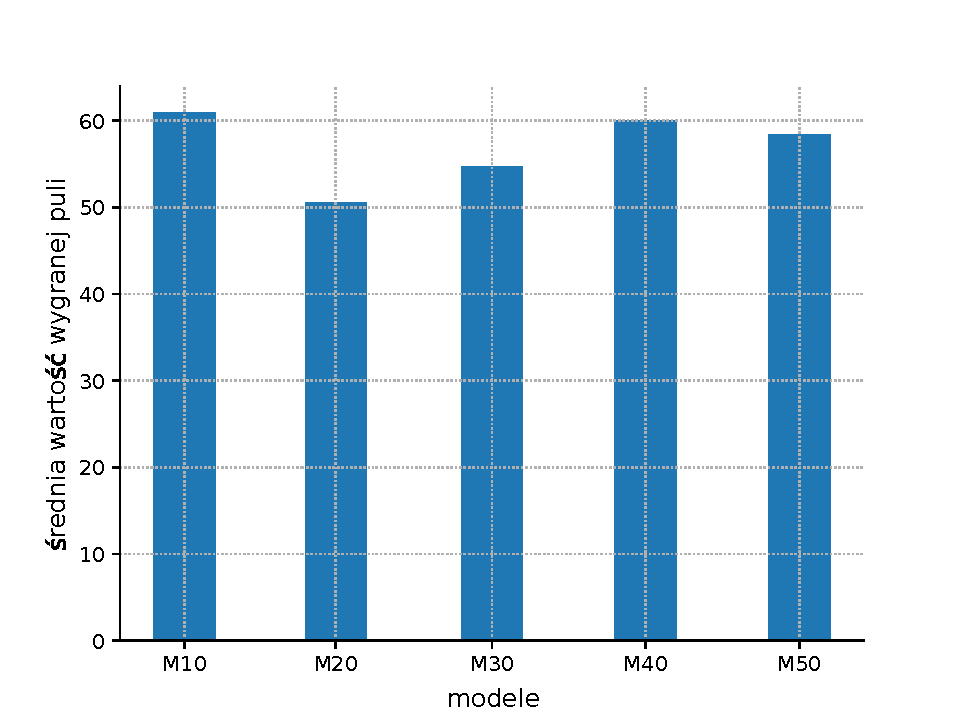
\includegraphics[width=0.75\textwidth]{./img/mecze_pw.pdf}
  \caption{Uśrednione wartości wygrywanych żetonów przez modele.}
\end{figure}


\begin{figure}[!ht]
  \centering
  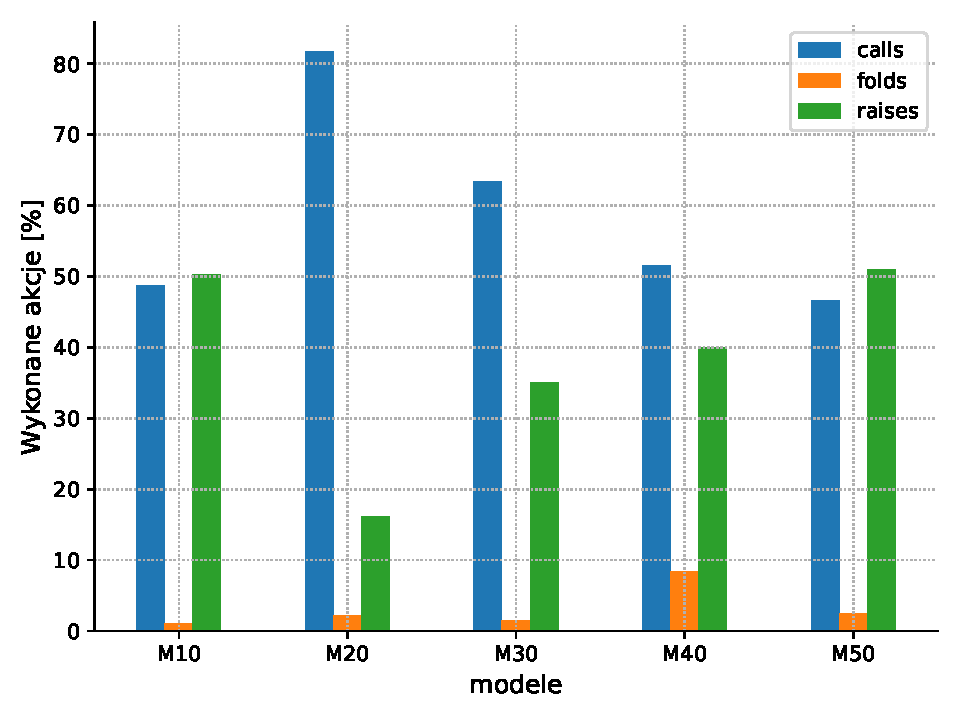
\includegraphics[width=0.75\textwidth]{./img/akcje.pdf}
  \caption{Rozkład wybieranych akcji przez modele podczas gry.}
\end{figure}

\begin{table}[th!]
\centering
\caption{Dokładne wyniki uśrednionych wartości zdobywanych lub traconych żetonów przez modele.}
\begin{tabular}{|c|c|c| }
   \hline
   model & średnia wygrana & średnia przegrana \\
    \hline
   1 & 61 & 65 \\ 
   \hline
   2 & 49 & 52  \\  
   \hline
   3 & 53 & 58 \\
   \hline
   4 & 61 & 50 \\
   \hline
   5 & 60 & 61 \\
   \hline
\end{tabular}
\end{table}

\newpage
\section{Porównanie modeli z programem HP}

Końcowym etapem oceny jakości algorytmu Deep CFR jest wykonanie gry między najlepszymi
utworzonymi
modelami a graczem HP (\emph{HonestPlayer}). Jest to program symulujący grę w HULH, wykonując tylko 
akcje opierające się na sile dostępnych kart.
W tym celu wykorzystano funkcję 
\emph{estimate\_hole\_card\_win\_rate} \cite{PPE}. Wykonuje ona określoną liczbę iteracji 
mozliwych wersji gier, a
nastepnie liczy szanse wygrania z dostepnymi kartami. W zalezności od zwracanej wartości
nastepnie wykonuje akcję \emph{fold} lub \emph{call}. 

Rozegrano 2 gry po 200 powtórzeń, gdzie każda z nich składała się z maksymalnie 10 rund.
Na rys. 4.10, 4.11, 4.12, 4.13 zaprezentowano
wyniki uzyskanych rozgrywek. Pierwszy z wykresów przedstawia częstotliwośc wygrywania modeli z
graczem HP. Wyniki pokazują ogromną przewagę utworzonych modeli z prostym programem.
Pomimo tego, analizując następne wykresy
można zauwazyć, że gracz HP wygrywa wiekszą średnią pulę względem modeli i przegrywa  
mniejszą stawkę. Prawdopodobnie wynika to z faktu wykonywania bardzo często ackji \emph{fold} oraz
\emph{call}. Jak widać taka strategia nie jest dobrym rozwiązaniem przez częste tracenie szansy na
wygraną.




\begin{figure}[!ht]
  \centering
  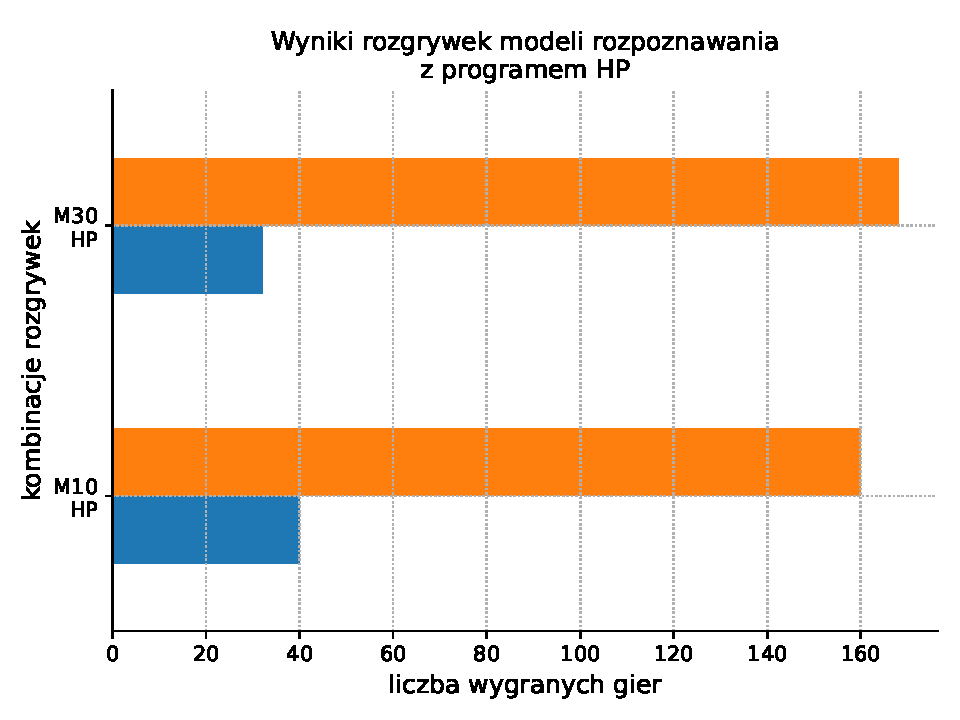
\includegraphics[width=0.7\textwidth]{./img/honest1.pdf}
  \caption{Wyniki rozgrywek między modelami M10, M30 i graczem HP.}
\end{figure}



\begin{figure}[!ht]
  \centering
  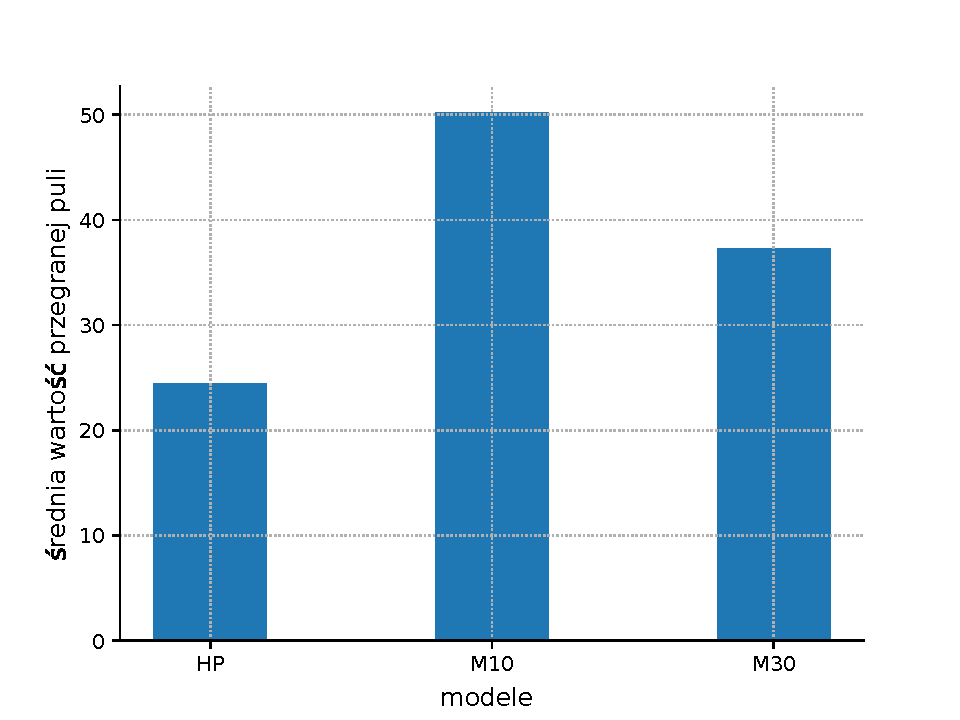
\includegraphics[width=0.7\textwidth]{./img/honest2.pdf}
  \caption{Wyniki przegrywanych pul między modelami M10, M30 i HP.}
\end{figure}

\begin{figure}[!ht]
  \centering
  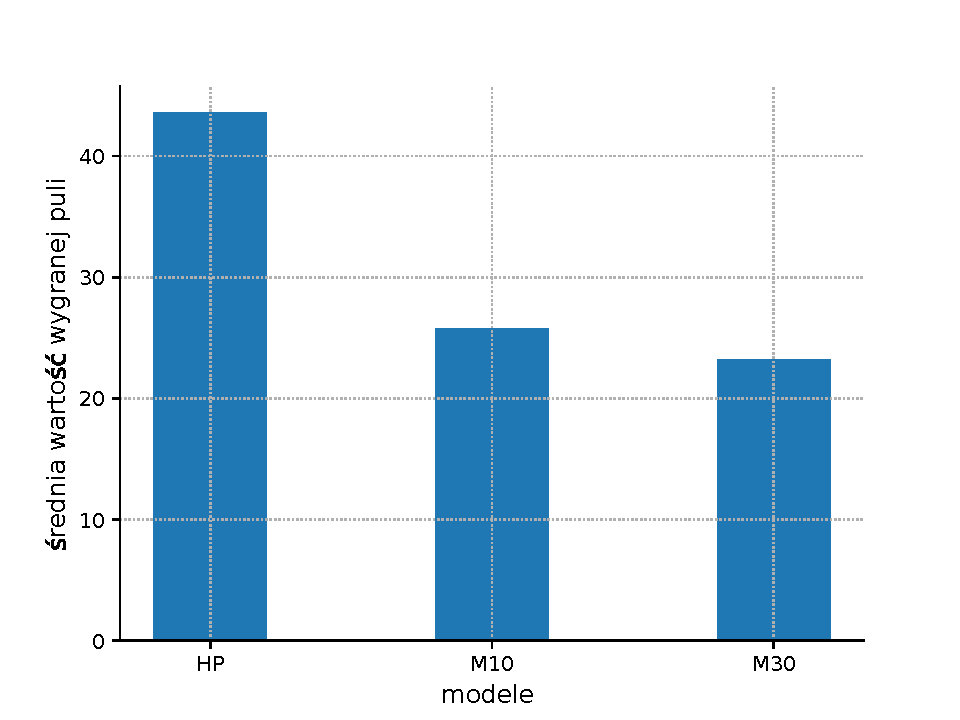
\includegraphics[width=0.75\textwidth]{./img/honest3.pdf}
  \caption{Wyniki wygrywanej pul między modelami M10, M30 i graczem HP.}
\end{figure}


\begin{figure}[!ht]
  \centering
  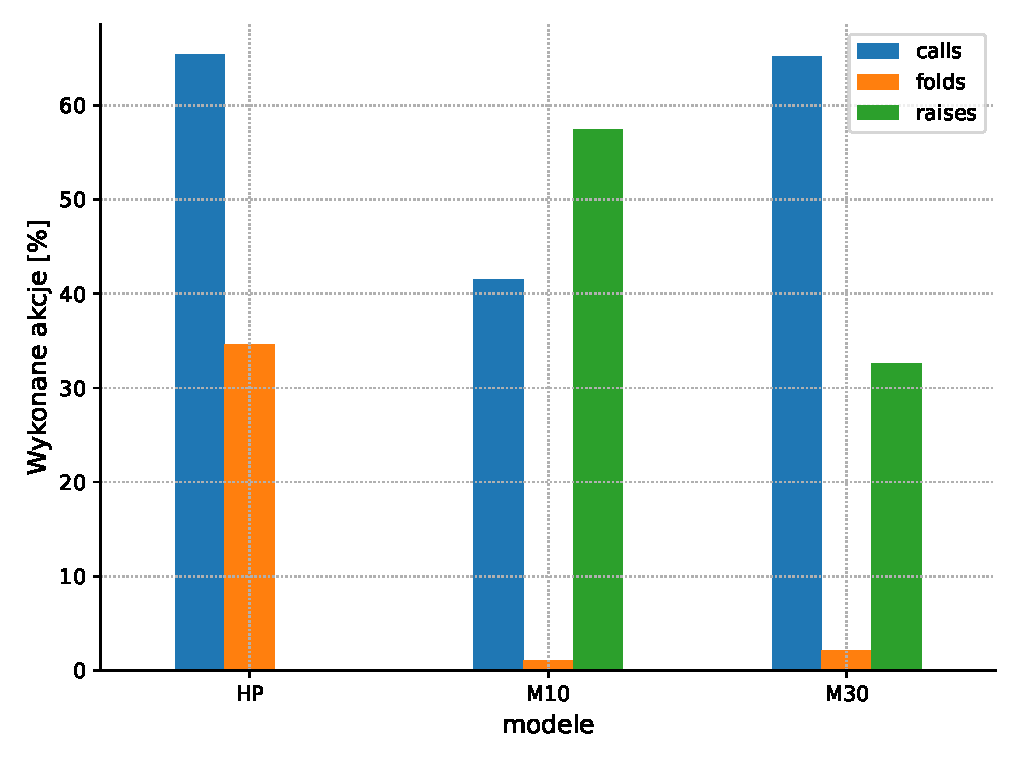
\includegraphics[width=0.75\textwidth]{./img/honest4.pdf}
  \caption{Rozkład wykonywanych akcji przez modele w trakcie rozgrywek.}
\end{figure}


\newpage
\text{}
\section{Podsumowanie}


Rozdział przedstawił wyniki utworzonych AI. Rezultaty okazały się mało optymistyczne. Model
wytrenowany w ostatniej iteracji nie uzyskuje najlepszych wyników, a przedostatnie AI przegrywa
najczęściej. Pomimo tego utworzony zbiór AI gra lepiej od prostych programów jak zaimplementowany 
gracz HP. Dodatkowo zauważono, że strategia polegająca na wykonywaniu tylko akcji \emph{call} i
\emph{fold} nie daje dobrych rezultatów. 

Model M10, który wygrywał najczęściej, posiada zrównoważony
rozkłąd wykonywanych akcji \emph{call}, \emph{raise} oraz bardzo rzadko pasuje grę. Dodatkowo z
taka strategią uzyskał najbardziej skrajne wyniki uśrednionych pul wygrywanych i przegrywanych
spośród utworzonych modeli. Korzystając z informacji zawartych w rozdziale 2, można
sklasyfikować graczy na bazie ich rozkładów akcji. Wszystkie AI oprócz modelu M40 wykonywały
bardzo rzadko akcję \emph{fold}, co oznacza, że wchodziły prawie zawsze do gry.
Dodatkowo modele M20 i M30 wykonywały często akcję \emph{call}, a M10 i M50 częściej
\emph{raise}. Średnia pula tracona przez te obiekty była powyżej 45 żetonów.
Oznacza to, że można je prawdopodobnie sklasyfikować do 
grupy pomiędzy Loose Passive i Loose Aggressive.


\chapter{Wnioski i podsumowanie etapów pracy}

Praca przedstawiła problem uczenia przez wzmacnianie w środowiskach częściowo obserwowalnych. 
Rozdziały 1 i 2 omówiły źródło takich problemów oraz poziom skomplikowania gry Poker Texas Hold'em.
Pokazały, że należy 
korzystać ze skomplikowanych algorytmów, które potrafią powiązać obserwacje z najlepszymi akcjami w
danym stanie. W przypadku gier karcianych w tym celu korzysta się z algorytmów bazujących na
metodzie CFR. 

Zaimplementowany algorytm w niniejszej pracy, Deep CFR usprawnił proces znany w metodzie CFR,
przez użycie sieci
neuronowych. Taka konstrukcja przyspiesza zbieganie się AI w dużych grach jak HULH
do Równowagi Nasha \cite{DCFR}.
Program użyty w pracy nie pozwolił na określenie stopnia bliskości
do takiego
stanu. Wynika to z faktu, że algorytmy używające metody CFR korzystają z metryki
\emph{Exploaibility} bazującej na wartości BR (\emph{Best Response})  do śledzenia postępów wybieranych
strategii przez AI \cite{lbr}.
Taki element głównie się implementuje w grach
abstrakcyjnych z powodu bardzo dużej obciążalności obliczeniowej. 
Duże gry stosują mniej dokładną metryki jak LBR(\emph{Local Best Response}),
która z dużym przybliżeniem zwraca stopień bliskości
modelu do Równowagi Nasha \cite{lbr}. Charakteryzują się one dużym skomplikowaniem 
implementacyjnym.

 
Z tego powodu do oceny jakości Deep CFR użyto prostszej metody.
Rozegrano wiele gier HULH między utworzonymi modelami, a następnie przeanalizowano wyniki
i wybrano
najlepszego z nich na bazie uzyskanych cech. Rezultaty okazały się mało optymistyczne w porównaniu
do czasu poświęconego na czas uczenia modeli.
Aktualny rozdział przedstawia możliwe przyczyny takich efektów oraz wnioski po dokonaniu wszystkich poprzednich etapów
pracy wraz z
mozliwymi poprawami parametów. Końcowa cześć pracy przedstawi dalszą historią algorytmu Deep CFR.
Dodatkowo zostanie przedstawiony 
możliwy
kierunek rozwoju uczenia maszynowego w środowiskach częściowo-obserwowalnych.





\section{Wnioski}

Gra Limit Poker Texas Hold'em jest bardzo trudnym środowiskiem do uczenia sztucznych
inteligencji, wynika to z częściowej obserwowalności. 
Z tego powodu model Cepheus, zdolny pokonywać ludzi w takim środowisku powstał 
dopiero w 2015 roku. Od tamtej pory rozpoczął się nagły rozwój metod uczenia maszynowego 
coraz większych gier 
karcianych.
Przykładami są DeepStack, Libratus lub Pluribus rozwiązujące grę Heads Up No Limit Texas Poker Hold'em i pokonujące
profesjonalnych ludzi.

Głównym zadaniem niniejszej pracy była próba zmierzenia się z takim środowiskiem. W celu uproszczenia
zadania wybrano grę HULH. Następnie zaimplementowano 
nowoczesny algorytm Deep CFR i wytrenowano pięć modeli
rozpoznawania. Pierwszy problem, jaki napotkano to, powolna nauka sieci $\theta_{p}$,
wraz z dużym błędem predykcji. Podczas uczenia wartości nie spadały poniżej 600.
Możliwym rozwiązaniem jest zwiększenie parametru \emph{learning rate}  
 oraz
dopracowanie architektury sieci neuronowej co przyczyni się do niewpadania wartości w minima
lokalne. Dodatkową przyczyną takich rezultatów mogą być
zbiory danych o słabej jakości. Prawdopodobnie nauka by przebiegała lepiej przez zwiększenie
zawartości obserwowalnych informacji wejściowych np. liczba żetonów w grze. W taki sposób
sieć neuronowa by miała więcej informacji, które by zostały użyte do zwracania właściwego 
wektora $D_{p}^{t}$.

Kolejnym problemem, który może mieć duże
znaczenie w grze to konstrukcja wprowadzanych informacji do modelu.
Dane wejściowe użyte w implementacji to karty widziane od strony gracza oraz historia 
z jednej rundy. Wadą takiej architektury jest to, że w praktyce rozgrywki Poker Texas Hold'em 
mogą odbywać się dłużej. Wtedy gracz musi dodatkowo używać takich informacji jak, wybrana strategia
przeciwnika w poprzednim etapie, czy grał ostrożnie, agresywnie albo blefował. Kolejnym czynnikiem jest 
sposób zmieniania się gry zależnie od liczby pozostałych żetonów w puli oraz od numeru rundy. Gracze
mogą podejmować bardziej ryzykowne i nierozważne ruchy, będąc w stanie bliskim porażki. Takie
informacje mogłyby być kluczowe w osiągnięciu zwycięstwa.
Prawdopodobnie przy uwzględnieniu tych elementów w sieci neuronowej, utworzone modele lepiej by
dobierały strategie do określonych stanów gry. To by wymagało wykonywania eksploracji MCCFR ES na znacznie większych drzewach decyzyjnych
obejmujących wiele rund. Dodatkowo dane wejściowe sieci neuronowej byłyby większe.
W takim przypadku
możliwym zbiorem informacji mógłby być zestaw składający się z widocznych kart, historii z wielu
rund, liczby żetonów każdego z graczy oraz numeru gry. W taki sposób model nauczyłby się 
lepiej dostosowywać sposób gry do obserwacji. 


Deep CFR spełnił funkcję i utworzył modele, które wygrywają z prostymi programami symulującymi
grę Poker Texas Hold'em jak przedstawiony gracz nieblefujący, HP w rozdziale 4. Pomimo dobrych
rezultatów dużym problemem okazał się
proces powstawiania sztucznych inteligencji. Pozornie można by było oczekiwać, że
algorytm będzie tworzył lepsze AI wraz z dłuższym czasem działania. W pracy doszło do odwrotnej
sytuacji. Sztuczne inteligencje utworzone w iteracjach 10 i 30 wygrywały z późniejszymi obiektami.
Ciężko określić przyczynę takich rezultatów. Pomocne okazałoby się użycie metryki
$\emph{Exploiability}$ do śledzenia postępów AI pomimo zwiększenia wymaganej mocy obliczeniowej
przez algorytm. Taki element pozwoliłby na stwierdzenie czy algorytm ominął punkt o najlepszej
jakości i w dalszym procesie uzyskuje podobne lub coraz gorze efekty. Pozwoliło by to na zatrzymanie procesu 
uzyskując najlepszy możliwy model z implementacji.







\section{Dalszy rozwój algorytmów bazujących na metodzie CFR}

Algorytm powstały w 2017 roku dawał dobre rezultaty, ale przez wykorzystanie dwóch sieci neuronowych
tworzył dużą wariancję wyników \cite{SD-CFR}. Z tego powodu powstał jego następca Single Deep CFR.
Po wykonanych testach uzyskał nie znacznie lepsze wyniki. Algorytm dalej nie był perfekcyjny, z tego
powodu w 2020 roku powstała metoda uczenia maszynowego o nazwie DREAM \cite{DREAM}. 
Jest to bardzo
dobry sposoby na tworzenie AI w środowiskach częściowo-obserwowalnych.
Pomimo tego wadą takich algorytmów 
jest to, że wymagają od gry,
aby wartość wygranej i przegranej sumowała się do zera. 
Taką cechą określa się środowiska zero-sum
\cite{DCFR}. Przez to algorytmy są mało adaptacyjne do innych środowisk.  
Kolejnym problemem tych
metod jest przeprowadzenie testów schodzenia się do Równowagi Nasha tylko w grach 2-osobowych \cite{DCFR}.
Wiele środowisk jak Poker Texas Hold'em standardowo uwzględnia większą ilość uczestników. Ten
problem udało się rozwiązać przez model Pluribus dopiero w 2019 roku. Na
podstawie takich informacji można stwierdzić, że zaimplementowany Deep CFR wraz z jego następcami nie
wyczerpały tematu środowisk gier karcianych. Nawet nowsze AI, które pokonują profesjonalnych
graczy jak DeepStack lub Libratus muszą trzymać się tych warunku \cite{libratus} \cite{ds}. 
Oznacza to, że takie gry to bardzo trudne środowiska, które prawdopodobnie będą jeszcze
długo badane pod względem możliwych rozwiązań.





\begin{thebibliography}{100}
   \bibitem{hist AI} Haenlein, Michael, and Andreas Kaplan. "A brief history of artificialintelligence: On the past, present, and future of artificial intelligence." California management review 61.4 (2019): 5-14.
   \bibitem{Dota2} Berner, Christopher, et al. "Dota 2 with large scale deep reinforcement learning." arXiv preprint arXiv:1912.06680 (2019).

   \bibitem{DCFR} Brown, Noam, et al. "Deep counterfactual regret minimization." International conference on machine learning. PMLR, 2019. 
   \bibitem{XFP} Heinrich, Johannes, Marc Lanctot, and David Silver. "Fictitious self-play in extensive-form games." International conference on machine learning. PMLR, 2015.
   \bibitem{CFR} Zinkevich, Martin, et al. "Regret minimization in games with incomplete information." Advances in neural information processing systems 20 (2007): 1729-1736.
   \bibitem{NFSP} Heinrich, Johannes, and David Silver. "Deep reinforcement learning from self-play in imperfect-information games." arXiv preprint arXiv:1603.01121 (2016).

   \bibitem{poker} Teófilo, Luís Filipe Guimarães. "Building a poker playing agent based on game logs using supervised learning." (2010).
   \bibitem{class} Félix, Dinis Alexandre Marialva. "Artificial intelligence techniques in games with incomplete information: opponent modelling in Texas Hold'em." (2008).
   \bibitem{mdp} Xiang, Xuanchen, and Simon Foo. "Recent Advances in Deep Reinforcement Learning Applications for Solving Partially Observable Markov Decision Processes (POMDP) Problems: Part 1—Fundamentals and Applications in Games, Robotics and Natural Language Processing." Machine Learning and Knowledge Extraction 3.3 (2021): 554-581.

   \bibitem{rn}  Nogal-Meger, P. (2012). Dylemat więźnia jako przykład wykorzystania teorii gier. Prace i Materiały Wydziału Zarządzania Uniwersytetu Gdańskiego, 10(4, cz. 2), 87–95.
   \bibitem{cepheus} Bowling, Michael, et al. "Heads-up limit hold'em poker is solved." Communications of the ACM 60.11 (2017): 81-88.
   \bibitem{libratus} Brown, Noam, and Tuomas Sandholm. "Superhuman AI for heads-up no-limit poker: Libratus beats top professionals." Science 359.6374 (2018): 418-424.
   \bibitem{ds} Moravčík, Matej, et al. "Deepstack: Expert-level artificial intelligence in heads-up no-limit poker." Science 356.6337 (2017): 508-513. 
   \bibitem{mccfr} Lanctot, Marc, et al. "Monte Carlo sampling for regret minimization in extensive games." Advances in neural information processing systems 22 (2009): 1078-1086.
   \bibitem{early} Prechelt, Lutz. "Early stopping-but when?." Neural Networks: Tricks of the trade. Springer, Berlin, Heidelberg, 1998. 55-69.

   \bibitem{lbr} Lisy, Viliam, and Michael Bowling. "Eqilibrium approximation quality of current no-limit poker bots." Workshops at the Thirty-First AAAI Conference on Artificial Intelligence. 2017.
   \bibitem{SD-CFR} Steinberger, Eric. "Single deep counterfactual regret minimization." arXiv preprint arXiv:1901.07621 (2019).
   \bibitem{DREAM} Steinberger, Eric, Adam Lerer, and Noam Brown. "DREAM: Deep regret minimization with advantage baselines and model-free learning." arXiv preprint arXiv:2006.10410 (2020).
   \bibitem{Pluribus} Brown, Noam, and Tuomas Sandholm. "Superhuman AI for multiplayer poker." Science 365.6456 (2019): 885-890.
   \bibitem{PPE} \text{https://github.com/ishikota/PyPokerEngine} GitHub.GitHub repository.
   \bibitem{tensorflow} Martín Abadi, Ashish Agarwal, Paul Barham, Eugene Brevdo,
Zhifeng Chen, Craig Citro, Greg S. Corrado, Andy Davis,
Jeffrey Dean, Matthieu Devin, Sanjay Ghemawat, Ian Goodfellow,
Andrew Harp, Geoffrey Irving, Michael Isard, Rafal Jozefowicz, Yangqing Jia,
Lukasz Kaiser, Manjunath Kudlur, Josh Levenberg, Dan Mané, Mike Schuster,
Rajat Monga, Sherry Moore, Derek Murray, Chris Olah, Jonathon Shlens,
Benoit Steiner, Ilya Sutskever, Kunal Talwar, Paul Tucker,
Vincent Vanhoucke, Vijay Vasudevan, Fernanda Viégas,
Oriol Vinyals, Pete Warden, Martin Wattenberg, Martin Wicke,
Yuan Yu, and Xiaoqiang Zheng.
TensorFlow: Large-scale machine learning on heterogeneous systems,
2015. Software available from tensorflow.org.
\end{thebibliography}



\end{document}

